\documentclass[a4paper,12pt]{article}


% add more packages if necessary
\usepackage{xspace}
\usepackage{graphicx}
\usepackage{xcolor}
\usepackage{hyperref}
\usepackage{epstopdf}

% TODO: Add your group name
\newcommand{\groupname}{Badgers\xspace}


\title{
Project Report \\ 
Group \groupname \\
\vspace{5mm}
\large Java and C\# in depth, Spring 2013
}
\author{
% TODO: Add your names here
Thomas Frick (03-150-927)\\
Matthias Ganz (04-862-850)\\
Philipp Rohr (04-397-030)
}
\date{\today}

\begin{document}
\maketitle


\section{Introduction}

This document describes the design and implementation of the \emph{Personal
Virtual File System} of group \emph{\groupname}. The project is part of the
course \emph{Java and C\# in depth} at ETH Zurich. The following sections
describe each project phase, listing the requirements that were implemented and
the design decisions taken. The last section describes a use case of using the
\emph{Personal Virtual File System}.

% PART I: VFS CORE
% --------------------------------------

\section{VFS Core}

VFS Core is a library that provides an implementation of a virtual file system.
The API that a client of this library can use consists of three interfaces that
are described in \ref{sec:coreClasses}. The VFS Core provides functionality to
create/open/dispose new virtual disks and allows the management of files and
directories within such a disk. Furthermore it provides a simple way to
import/export files from/to the host file system.

The library internally works with a virtual disk that is divided into a header,
index and data section, having the index represented as B-tree. Such a design
allows quick access to the data on the disk.


\subsection{Requirements}
Below one will find a list of the requirements implemented in this project.

\subsubsection {disk management}
\begin{itemize}
  \item \emph{The virtual disk must be stored in a single file in the working
  directory in the host file system.}
  \item \emph{VFS must support the creation of a new disk with the specified
  maximum size at the specifieed location in the host file system. }
  \item \emph{VFS must support several virtual disks in the host file system.}
  \item \emph{VFS must support disposing of the virtual disk.}
  \item \emph{VFS must support querying of free/occupied space in the virtual
  disk.}
\end{itemize}  These requirements are met with the classes
\begin{verbatim}
ch.eth.jcd.badgers.vfs.core.VFSDiskManagerImpl
ch.eth.jcd.badgers.vfs.core.config.DiskConfiguration
\end{verbatim} allow creation/deletion and opening of the disk on the host
file system. Clients of the library have to pass a \textit{DiskConfiguration}
to the \textit{VFSDiskManagerImpl} when calling \textit{create} or
\textit{open}
\subsubsection{file management}
\begin{itemize}
  \item \emph{VFS must support creating/deleting/renaming directories and files.}
  \item \emph{VFS must support navigation: listing of files and folders, and
  going to a location expressed by a concrete path.}
  \item \emph{VFS must support moving/copying directories and files, including
  hierarchy.}
  \item \emph{VFS must support importing files and directories from
  the host file system.}
  \item \emph{VFS must support exporting files and directories to the host file
  system.}
\end{itemize} These requirements are met with the classes
\begin{verbatim}
ch.eth.jcd.badgers.vfs.core.VFSEntryImpl
ch.eth.jcd.badgers.vfs.core.VFSPathImpl
ch.eth.jcd.badgers.vfs.core.VFSFileInputStream
ch.eth.jcd.badgers.vfs.core.VFSFileOutputStream
\end{verbatim}The \textit{VFSEntryImpl} allows
copy, move (and rename), delete, listing of children and going to the parent
(navigation). Together with the streams it also supports importing/exporting
to any location clients of the vfs library wish to. The classes
\begin{verbatim}
ch.eth.jcd.badgers.vfs.ui.VFSConsole
ch.eth.jcd.badgers.vfs.ui.VFSUIController
\end{verbatim} demonstrate this by importing and exporting to the host file
system.

\subsubsection {bonus features}
\begin{itemize}
  \item \emph{Elastic disk: Virtual disk can dynamically grow or shrink,
  depending on its occupied space.}
\end{itemize}
The implementation only allows growing if more files are imported. Shrinking is
not supported.

\begin{itemize}
  \item \emph{Compression, if implemented with 3d party library.}
  \item \emph{Compression, if implemented by hand (you can take a look at
  the arithmetic compression)}
\end{itemize}

The classes
\begin{verbatim}
ch.eth.jcd.badgers.vfs.compression.BadgersLZ77CompressionInputStream
ch.eth.jcd.badgers.vfs.compression.BadgersLZ77CompressionOutputStream
ch.eth.jcd.badgers.vfs.compression.BadgersRLECompressionInputStream
ch.eth.jcd.badgers.vfs.compression.BadgersRLECompressionOutputStream
\end{verbatim}
implement streams that can be wrapped around \textit{VFSFileInputStream} and
\textit{VFSFileOutputStream}. The \textit{DiskConfiguration} allows
to switch compression on and to declare which algorithm shall be chosen. This
allows easy configuration of any 3d party compression streams (which was not
chosen to implement, because of the implementation of our own compression
algorithm).

\begin{itemize}
  \item \emph{Encryption, if implemented with 3d party library.}
  \item \emph{Encryption, if implemented by hand.}
\end{itemize}

The classes
\begin{verbatim}
ch.eth.jcd.badgers.vfs.encryption.CaesarInputStream
ch.eth.jcd.badgers.vfs.encryption.CaesarOutputStream
\end{verbatim}
show how encryption can be implemented in the library. It was chosen to
implement encryption similar to compression with streams, which allows easy
configuration via \textit{DiskConfiguration}. These streams are mainly for
demonstration how encryption should work and shall not be used in high
security environments :-)

\subsection{Design}
This section describes the main aspects of the VFS core library. It shows the
implementation of the core interfaces and classes, explains the mock classes and
tests and eventually describes the file format and its management classes.

\subsubsection{Core Classes}\label{sec:coreClasses}
Figure \ref{fig:core_classes} gives an overview of the main interfaces and
classes that were implemented. The interfaces \textit{VFSDiskManager},
\textit{VFSEntry} and \textit{VFSPath} can be used by clients using the library
implemented here.
\begin{itemize}
\item{\textit{VFSDiskManager}} The implementations of this interface provide
mainly a way to open, create and dispose new virtual disks. Additionally one can
get the root entry of the file system and get additional information about an
opened disk.
\item{\textit{VFSEntry}} Represents a directory or file on the file system. A
\textit{VFSEntry} provides all the required methods to manipulate files and
directories and importing/exporting files into the virtual file system. The
general meaning of \textit{VFSEntry} is, that such objects usually exist on the
filesystem.
\item {\textit{VFSPath}} Represents a path on the file system to a given
\textit{VFSEntry}. It has a slightly looser coupling to the file system as a
path does not imperatively need to exist.
\item {\textit{FindInFolderCallback}} The \textit{find} and
\textit{findInFolder} methods on \textit{VFSDiskManager} and \textit{VFSEntry}
require a callback object where the find mechanisms provided by the mock and the
real implementations will notify the caller when a new entry is found. So a
client can start the search asynchronously and can handle the notifications for
example with updating lists. The console implementation simply lists the
absolute paths to the found entries.
\end{itemize}

The intention of those interfaces is to hide the real implementation of the
virtual file system from a client. With that in mind it should be simple to add
a network layer upon the real implementation without changing client code. The
classes \textit{VFSDiskManagerImpl, VFSEntryImpl (and its descendants) and
VFSPathImpl} implement all the management for actually using the VFS on a virtual disk.

\begin{figure}[h!]
\centering
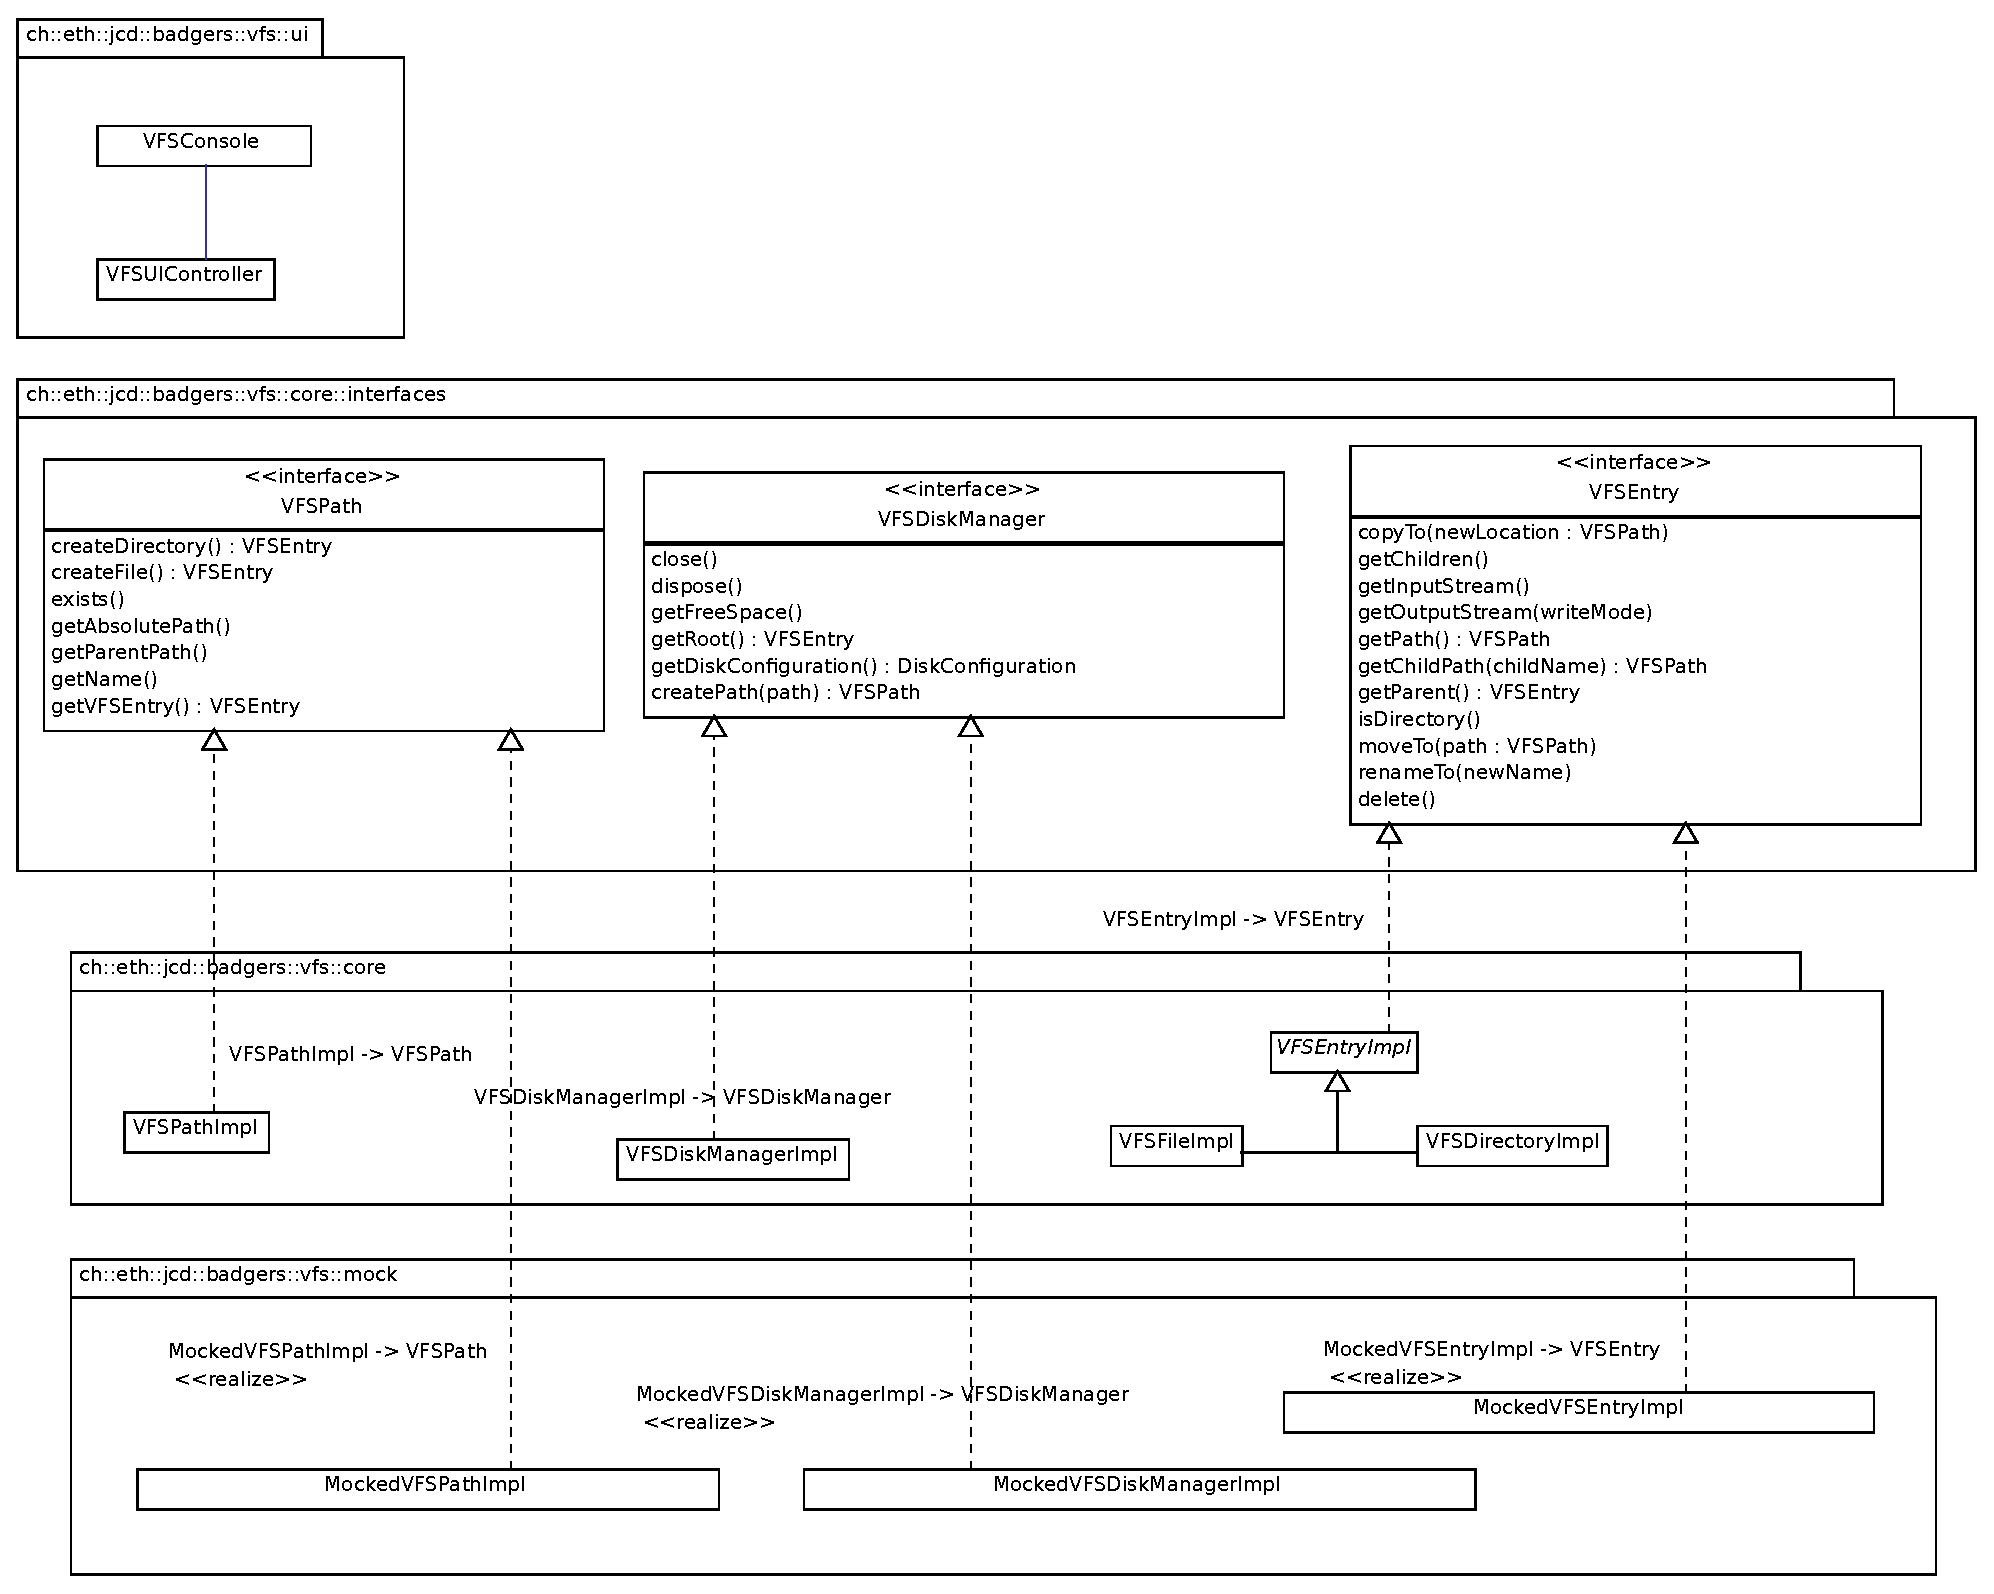
\includegraphics[width=1\textwidth]{figures/core_classes.eps}
\caption{core classes}
\label{fig:core_classes}
\end{figure}

\subsubsection{Design on compression and encryption}

Both compression and encryption is only applied to file content. 
Neither file names nor folder structure is encrypted. 
Encrypting the whole virtual disk would have greatly increased complexity of the virtual disk core.  
Considering project deadlines it was decided to only compress and encrypt file content.


\subsubsection{Mocking}
For discussing the semantics of the virtual file system and the development of 
the interfaces explained in \ref{sec:coreClasses} it was decided to implement a mock
that works against the host file system. The mock classes implement all
the interfaces and were very helpful for acquiring a common understanding of how
the interface shall be used by clients. In a further step it was very useful to have
the mock classes while developing the console application. Hence the console
could be developed independently from the real implementation.
\subsubsection{Test}
During the development a bunch of test cases came to life. The tests solely
depend on the interfaces and thus they can run against the mock classes and the
real implementation. This was a huge help in finding bugs in the slightly more
complicated real implementation.
\subsubsection{The \emph{real} implemenation}

Eventually some code was developed  that handles a virtual disk. This code and
some details about the file format are described in this section.

\paragraph{The classes}

Figure \ref{fig:vfs_impl_classes} shows the overview over the classes
implemented for the disk handling and file management.


\begin{figure}[h!]
\centering
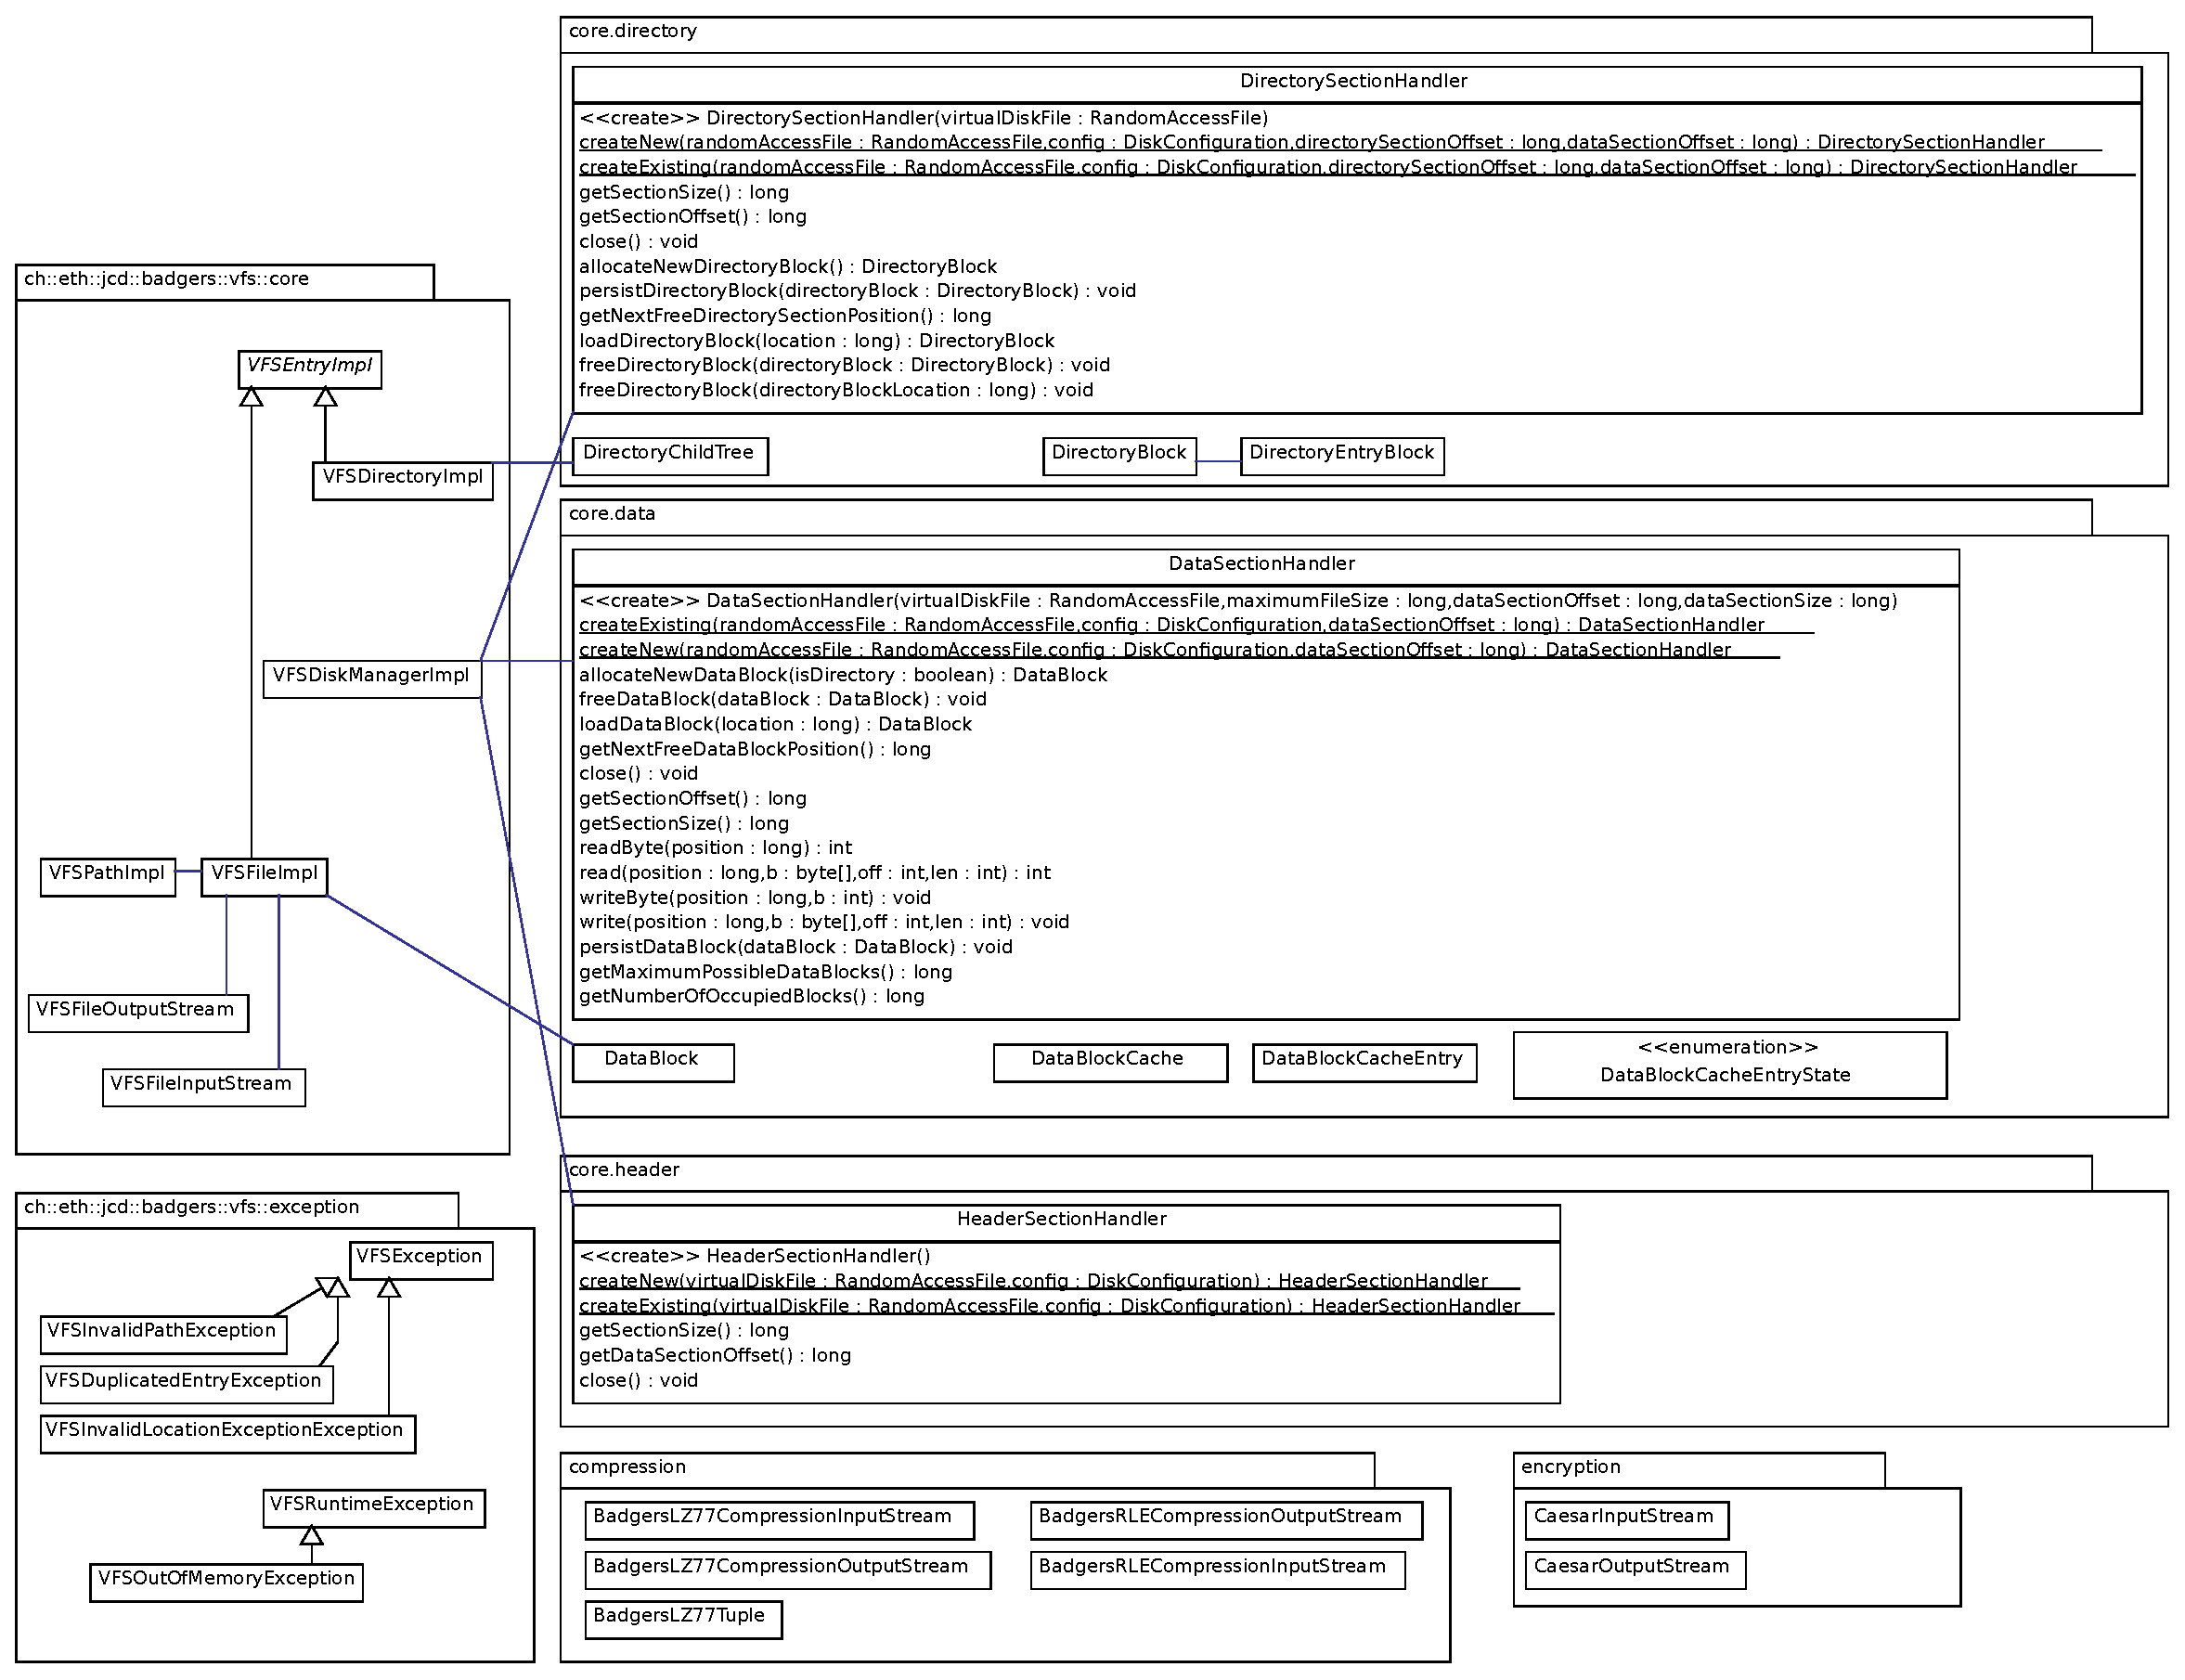
\includegraphics[width=1\textwidth]{figures/vfs_impl_classes.eps}
\caption{Implementation of the VFS core classes}
\label{fig:vfs_impl_classes}
\end{figure}

The classes were divided into several packages which are explained here in more
detail.

\subparagraph{core}
The \textit{core} package contains the implementation of the interfaces
mentioned in section \ref{sec:coreClasses}. Clients of the VFS core library operate on these
classes to manipulate the virtual file system.

\subparagraph{exception}
While manipulating the file system some exceptional behaviour might occur and
thus some exceptions will be thrown by the core classes. These exception are
propagated to the clients of the VFS core libraries.

\subparagraph{core.header}
As the virtual disk is divided into three sections (header, directory and data)
the classes that handle the management of the header section are put in the
package \textit{core.header}.
\subparagraph{core.data}
\textit{core.data} contains the classes that manipulate the data section on the
file system. This mainly means managing data blocks and actually writing/reading
the raw data bytes of files to the virtual disk.
\subparagraph{core.directory}
\textit{core.directory} contains the classes that manage the index of the file
system. That means that the whole directory structure is maintained in here.
This is done in a B-Tree that contains all references to directories and files
currently saved in the file system. More about the internals of directory
section can be found in section \ref{sec:file_format}

\subparagraph{encryption}
The encryption package shows some demo classes that implement a ceasar
cipher\footnote{http://en.wikipedia.org/wiki/Caesar\_cipher}. These classes are
mainly to show how encrpytion in VFS core can be implemented and configured. To
enable encryption in a new virtual disk one has to enable it in the
\textit{DiskConfiguration} that is passed to the \textit{VFSDiskManagerImpl} at
creation. Upon selecting the encryption algorithm the encryption streams will be
wrapped around the \textit{VFSFileInput- and VFSFileOutputStream}s.

\subparagraph{compression}

To reduce the data volume within the virtual disk, compression on each file can
be enabled. As mentioned earlier, compression is implemented as Input- and
OutputStreams and thus is wrapped around the \textit{VFSFileInput- and
VFSFileOutputStream}s. Currently available compression algorithms are run length
encoding \cite{rle} and LZ77 \cite{lz77}.

\begin{itemize}
  \item {\textit{Run Length Encoding}} The available 8bit run length
  encoding(rle) algorithm is a very simple form of data compression where
  multiple occurrence of the same byte were stored as a single byte value and
  the corresponding count. It is useful for simple graphic images like line
  drawings and icons.
  \item {\textit{LZ77}} Abraham Lempel and Jacob Ziv introduced the LZ77 lossless
  compression algorithm in 1977. Newer compression methods such as GZIP or DEFLATE often use LZ77-based
  algorithms. The compression is achieved by replacing the data with a reference
  to an earlier existing copy in the data input stream. For that a window of
  a certain size is held in memory where existing copies of the current data are
  searched.
\end{itemize}


\paragraph{The File Format}\label{sec:file_format}
This section describes the binary file format used by the file system inside a
virtual disk. The file is separated into three major parts. The header, index
and the data section. Each of them is described below. Figure
\ref{fig:disk_overview} gives an overview, of how the sections are distributed
in the virutal disks and what contents they have.

\begin{figure}[h!]
\centering
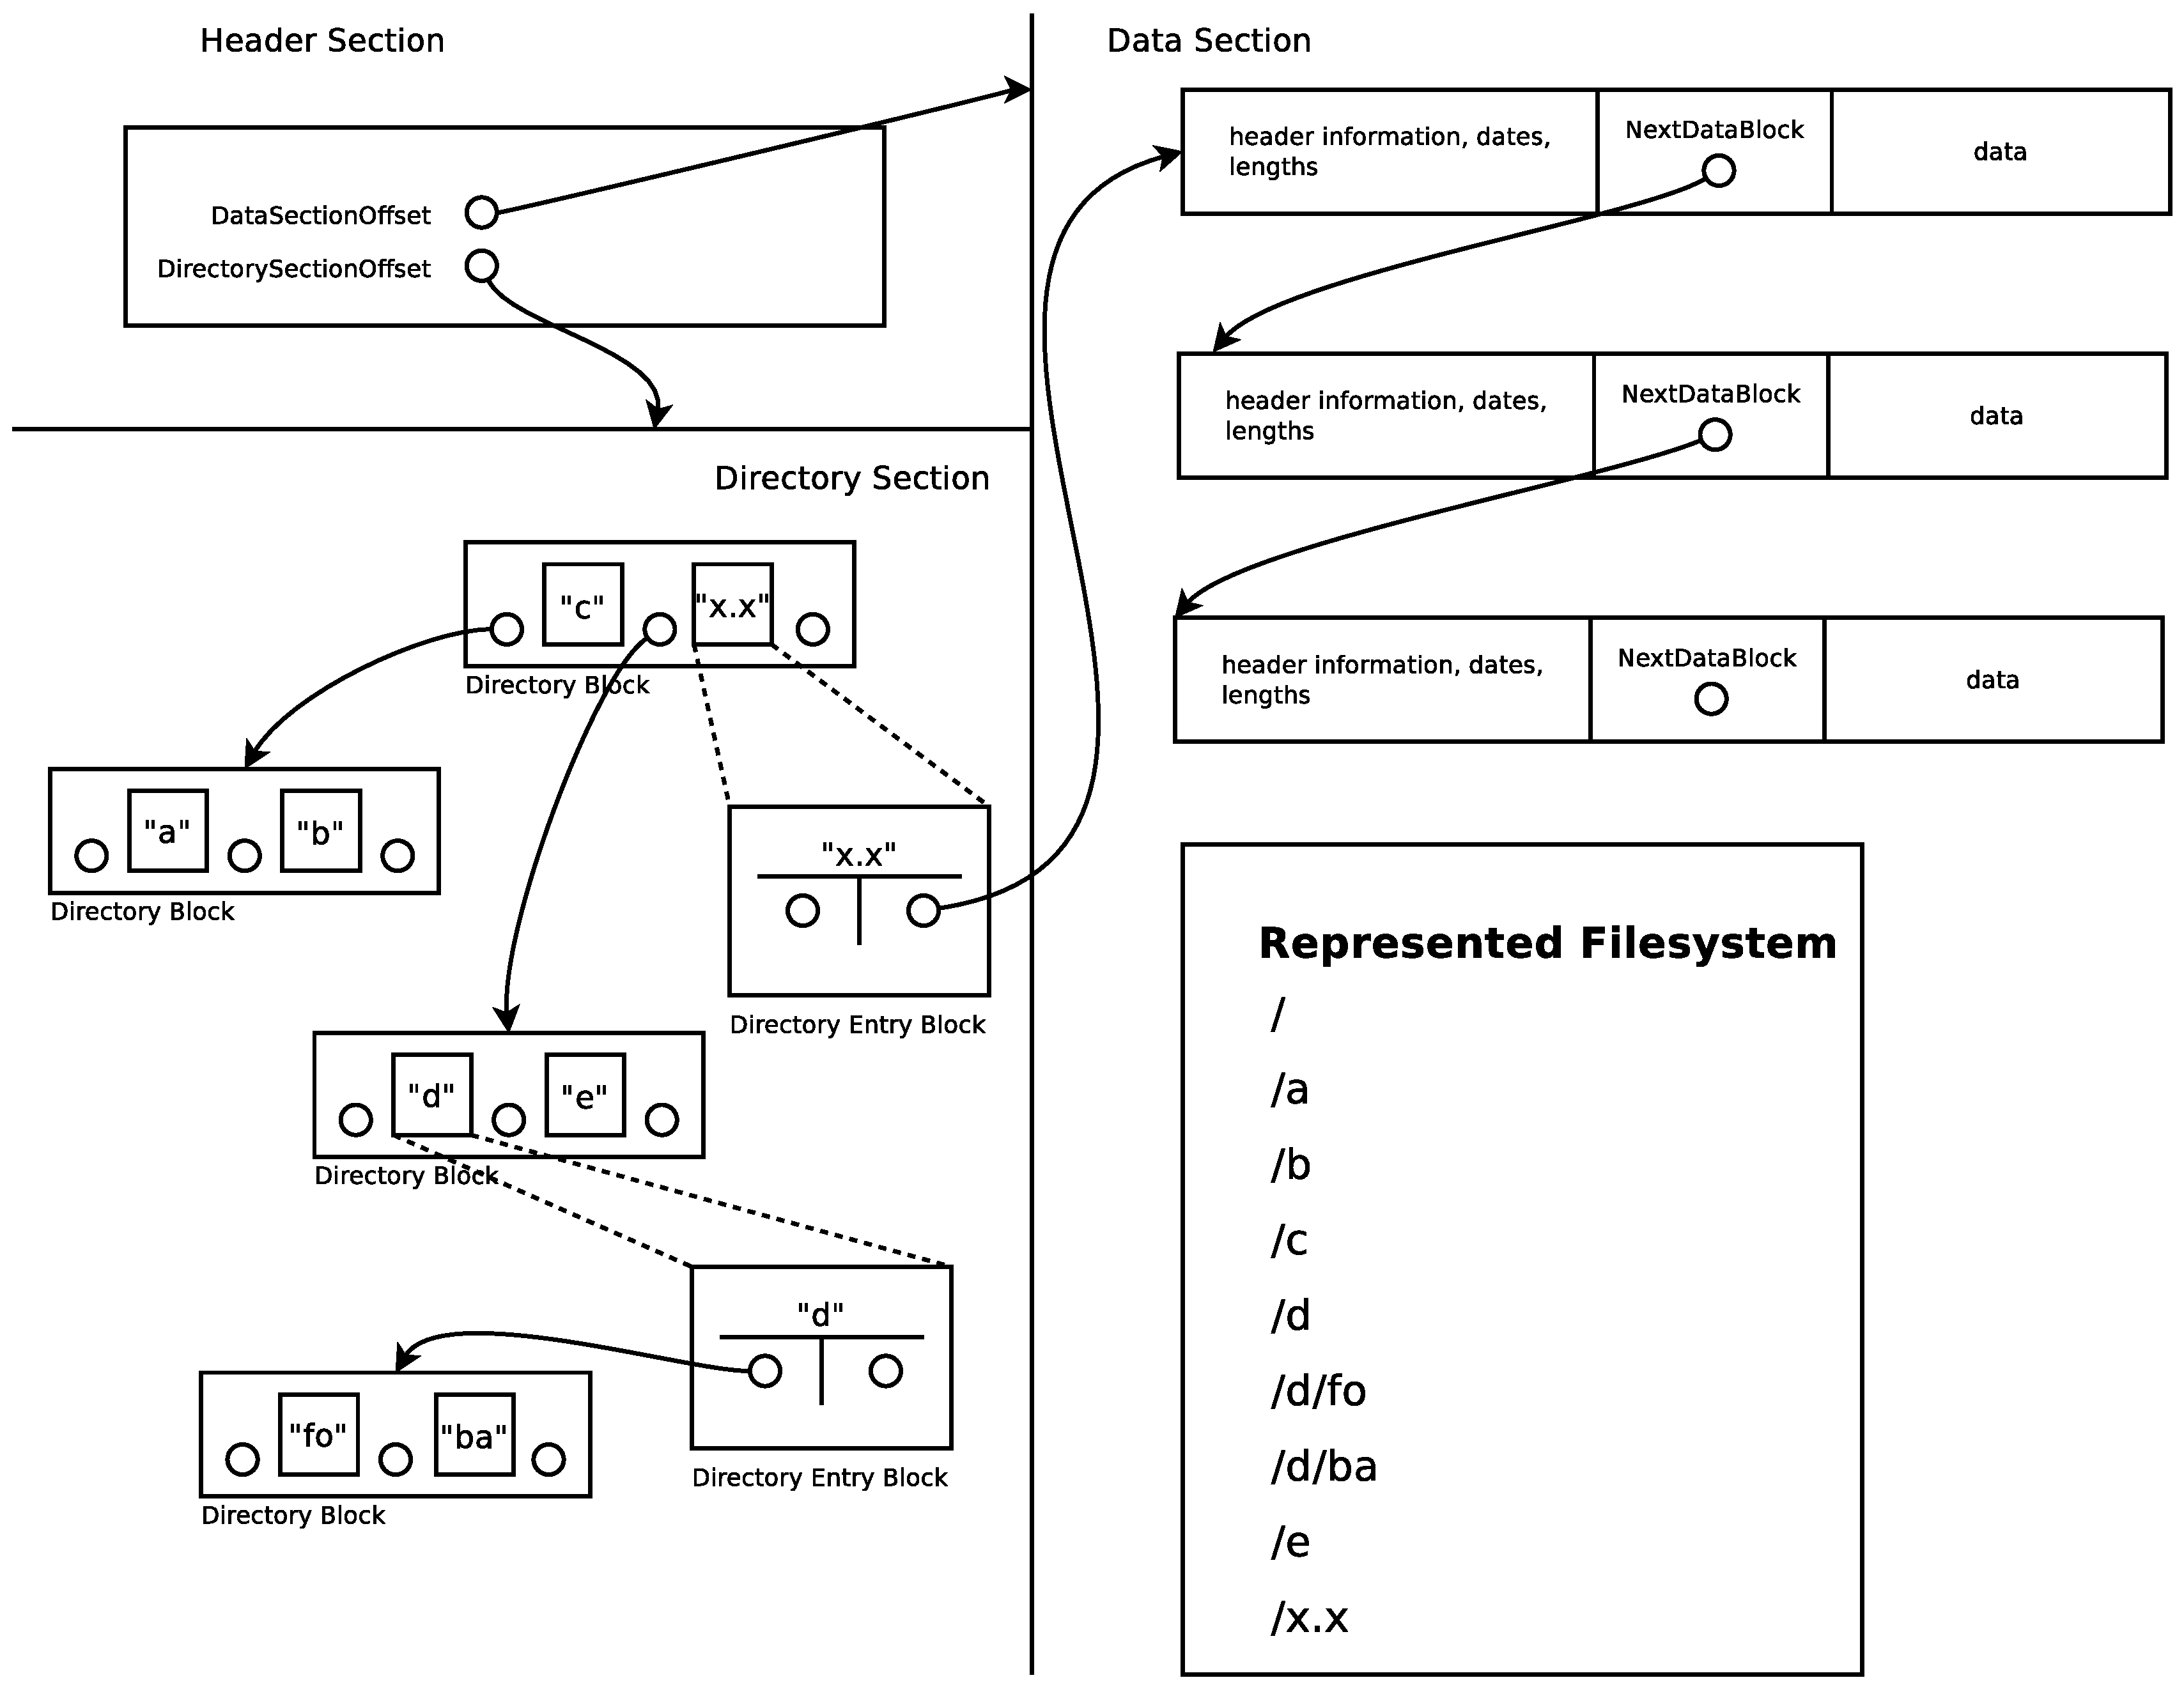
\includegraphics[width=1\textwidth]{figures/fileFormat.eps}
\caption{Overview of a disk}
\label{fig:disk_overview}
\end{figure}

\subparagraph{Header Section} The header section contains some general information
about the currently opened virtual disk. The details can be found in the
following table:

\begin{tabular}{|l|l|p{5cm}|}
\hline
\textbf{Name} & \textbf{Length} & \textbf{Description}
\\  \hline
Info & 50 byte UTF-8 String & Contains something like Badger VFS 2013
\\ \hline
Version & 10 byte UTF-8 String & Contains something like "1.0"
\\ \hline
Compression used & 20 byte UTF-8 String & null or indicates compression used for this file
\\ \hline
Encryption used & 20 byte UTF-8 String & null or indicates encryption used for this file
\\ \hline
DirectorySectionOffset & long (8 byte) &  File offset where the directory
section starts \\ \hline
DataSectionOffset & long (8 byte) &  File offset where our data section starts
\\ \hline
 SaltString & 8 bytes  & Salt used to hash username and password randomly string generated while creating this
   file. (Not implemented yet)
 \\ \hline
  Password & xxx bytes  & CryptoHash (SHA-whatever) of Password+SaltString  (Not implemented yet)
\\ \hline

\end{tabular}


\subparagraph{Directory Section}
The directory section describes which files and folders belong to which parent
directory. This section has a fixed size and contains so called
\textit{DirectoryBlocks} which also have a fixed size. This makes management and
manipulation easy. To each directory belongs a B-Tree structure which lists all
contained entries.


\subparagraph*{DirectoryBlock}

One \textit{DirectoryBlock} represents a node in the B-Tree of order 2.

\begin{tabular}{|l|l|p{5cm}|}
\hline
\textbf{Name} & \textbf{Length} & \textbf{Description}
\\  \hline

DirectoryHeader & 1 byte & Header information. This header makes it easy to
determine whether a \textit{DirectoryBlock} is in use or not (memory
management)

\\  \hline

DirectoryEntryBlock1 & 128 byte & The smaller key inserted into the
B-Tree

\\  \hline

DirectoryEntryBlock2 & 128 byte & The bigger key inserted into the B-Tree

\\  \hline

DirectoryBlockLink1 & 8 byte & Points to another DirectoryBlock which contains
keys smaller than DirectoryEntryBlock1

\\  \hline

DirectoryBlockLink2 & 8 byte & Points to another DirectoryBlock which contains
keys bigger than DirectoryEntryBlock1 but smaller than DirectoryEntryBlock2

\\  \hline

DirectoryBlockLink3 & 8 byte & Points to another DirectoryBlock which contains
keys bigger than DirectoryEntryBlock2

\\  \hline


\end{tabular}

\subparagraph*{DirectoryEntryBlock}

Represents a single directory or file.

\begin{tabular}{|l|l|p{5cm}|}
\hline
\textbf{Name} & \textbf{Length} & \textbf{Description}
\\  \hline

Filename & 112 byte & UTF-8 file name String


\\  \hline

DataBlockLocation & 8 byte & Pointer to a DataBlock located in the Data Section.
This DataBlock holds some meta information about the current directory


\\  \hline

DirectoryEntryTreeRoot & 8 bytes & Pointer to a DirectoryBlock located in the
Directory Section. This referenced DirectoryBlock is the Root Block of a B-Tree
containing all entries of that directory specified by the current Directory Entry Block.
\newline

\textbf{This field containing a 0 indicates that this entry represents a file not a directory}



\\  \hline

\end{tabular}


\subparagraph{Data Section}
The data section is split into blocks where each of them is 1024 bytes long.
Each block contains some amount of data and points to a subsequent block (Simple
linked list).\newline\newline
Block layout \\

\begin{tabular}{|l|l|p{5cm}|}
\hline
\textbf{Name} & \textbf{Length} & \textbf{Description}
\\  \hline
BlockHeader & 1 byte &
\\
\hspace{0.2cm} 0) Header-Bit (LSB) & &  If set to 1 this is the first DataBlock
of a file.
\\
\hspace{0.2cm} 1) not used & &
\\
\hspace{0.2cm} 2) not used & &
\\
\hspace{0.2cm} 3) not used & &
\\
\hspace{0.2cm} 4) not used & &
\\
\hspace{0.2cm} 5) not used & &
\\
\hspace{0.2cm} 6) not used & &
\\
\hspace{0.2cm} 7) not used & &

\\  \hline
NextDataBlock & 8 byte &
Points to the start address of the next DataBlock (linked list).
0 if this is the last DataBlock of a certain file or folder.
\\  \hline
CreationDate & 8 byte & UTC Time when this file was created
\newline \textit{This field only exists if Header-Bit is set to 1}
\\  \hline

DataLength & 4 byte &
Indicates the number of data saved on this DataBlock.

\\  \hline
Data & n byte & user data (may be encrypted/compressed)
\\  \hline
\end{tabular}


\paragraph{The root directory}

By definition the root directory's DataBlock and DIrectoryBlock are located at the very first position in their correspond sections.



% PART II: VFS Browser
% --------------------------------------

\section{VFS Browser}

VFS Browser is a JAVA Swing application atop the VFS core. The browser was
developed during the second milestone of the project. The main goal of the
browser application is to give users a convenient access to their virtual disks.
It allows browsing files and folders, as well as importing and
exporting from/to the host filesystems. Additionally it provides a convenient
search interface, that allows quick finding of files.


\subsection{Requirements}
Below one will find a list of the requirements implemented in this project.

\subsubsection {Basic Requirements}
\begin{itemize}
  \item \emph{The browser should be implemented on one of the following
  platforms: desktop, web or mobile}
  \item \emph{The browser should support all operations from Part 1 (VFS core).
  For example, users should be able to select a file/folder and copy it to
  another location without using console commands. }
  \item \emph{The browser should support both single and multiple selection of
  files/folders.}
  \item \emph{The browser should support keyboard navigation. The mandatory set of operations includes folder
  navigation, going to parent and child folders (this is optional for mobile applications due to limited
  keyboard functionality).}
  \item \emph{The browser should support mouse navigation (or touch in case of the mobile platform). The
  required operations are the same as in requirement 4.}
  \item \emph{The browser should support file-name search based on user-given
  keybwords. The search should provide options for: case sensitive/ case
  insensitive search; restrict search to folder; restrict search to folder and subfolders.}
\end{itemize}  These requirements are met with the classes
\begin{verbatim}
ch.eth.jcd.badgers.vfs.ui.desktop.view.BadgerMainFrame
ch.eth.jcd.badgers.vfs.ui.desktop.view.BadgerMenuBar
ch.eth.jcd.badgers.vfs.ui.desktop.view.BadgerTable
ch.eth.jcd.badgers.vfs.ui.desktop.view.DiskSpaceDialog
ch.eth.jcd.badgers.vfs.ui.desktop.view.ImportDialog
ch.eth.jcd.badgers.vfs.ui.desktop.view.NewDiskCreationDialog
\end{verbatim} provide the frontend functionalities to meet the requirements

\begin{verbatim}
ch.eth.jcd.badgers.vfs.ui.desktop.model.BadgerFileExtensionFilter
ch.eth.jcd.badgers.vfs.ui.desktop.model.EntryTableModel
ch.eth.jcd.badgers.vfs.ui.desktop.model.EntryUiModel
ch.eth.jcd.badgers.vfs.ui.desktop.model.ParentFolderEntryUiModel
\end{verbatim} are the model classes, that model table entries and ui models

\begin{verbatim}
ch.eth.jcd.badgers.vfs.ui.desktop.controller.BadgerController.java
ch.eth.jcd.badgers.vfs.ui.desktop.controller.BadgerViewBase.java
ch.eth.jcd.badgers.vfs.ui.desktop.controller.DesktopController.java
ch.eth.jcd.badgers.vfs.ui.desktop.controller.SearchController.java
ch.eth.jcd.badgers.vfs.ui.desktop.controller.WorkerController.java
\end{verbatim} provide the controller classes of a typical MVC design. 


\subsubsection {Implemented Bonus Requirements}
\begin{itemize}
  \item \emph{Responsive UI, i.e. the browser does not stall during long-running
  operations (i.e. file search or import).} Is implemented with decoupling the
  disk work from the gui work. This is done with a single thread accessing the
  disk api. This thread has a work queue to which \textit{Actions} are added.
  \item \emph{Advanced search; For example, search with wildcards.} For this the
  API had to be extended slightly.
  \item \emph{Drag-and-drop for manipulative operations (import).} For that we
  register a \textit{DropTarget} on the \textit{BadgerTable} that has a
  \textit{DropTargetListener} which starts the import on the
  \textit{DesktopController}.
\end{itemize}

\subsubsection {Not Implemented Bonus Requirements}
\begin{itemize}
  \item \emph{Nice-to-have features like operation progress report (e.g. the
  number of files processed during export) or drag-and-drop for manipulative
  operations (move, copy).}
  \item \emph{The browser is implemented for an additional platform}
  \item \emph{Efficient full-text search (using some sort of indexing).}
\end{itemize}

\subsection{Design}
This section describes the main aspects of the VFS Browser applicatoin. It shows
the implementation of the core interfaces and classes.

\subsubsection{GUI classes}\label{sec:guiClasses}
Figure \ref{fig:gui_classes} gives an overview of the main interfaces and
classes that were implemented for the gui. The implementation followed the rules
of a MVC design dividing the aspects of Model View and Control to their
respective classes. According to the partition of MVC the classes were
partitioned into the packages \textit{model, view and controller}.

\begin{figure}[h!]
\centering
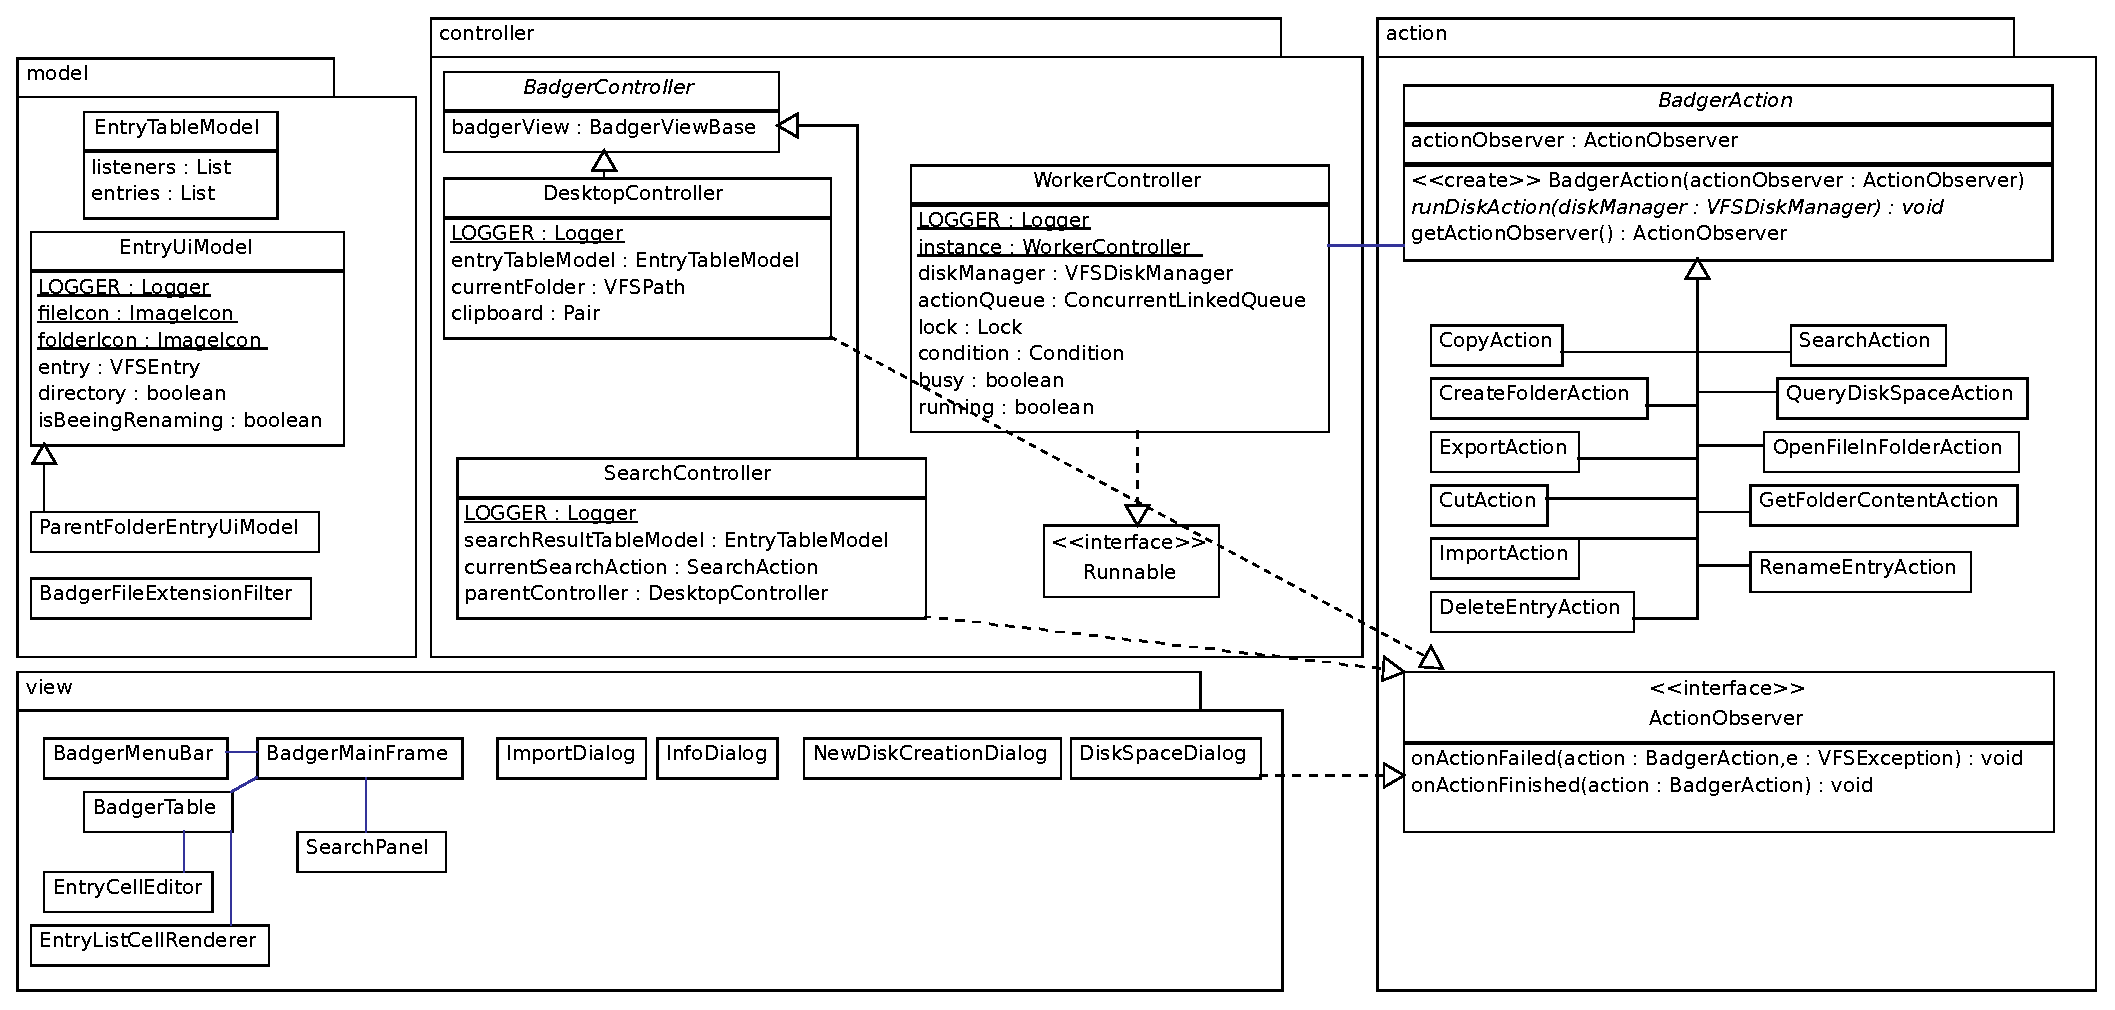
\includegraphics[width=1\textwidth]{figures/gui_classes.eps}
\caption{gui classes}
\label{fig:gui_classes}
\end{figure}


\subsubsection{Decoupling of GUI and working threads}
This section describes the way how the decoupling from GUI and working threads
was implemented. This decoupling mades the GUI still responsive even tough some
long running tasks like import or search would be running. Figure
\ref{fig:decouple_threads} shows the sequence diagram of the example ``Import'':
The \textit{DesktopController} which lives in the GUI thread creates a new
\textit{ImportAction} that is enqueued in the \textit{WorkerController}'s action queue. It is worth to mention, that the
\textit{WorkerController} is a singleton, that has an \textit{instance} field. The
\textit{WorkerController} has a thread that works on a blocking queue and every
time it gets a \textit{BadgerAction} the thread wakes up and performs the action
on the VFS core API. After the API work is done (in this case the import of
files), the \textit{WorkerController} calls the corresponding
\textit{ActionObserver}, which is in most cases the \textit{DesktopController}
instance, so that the GUI can be updated. This design ensures single threaded
access on the VFS core API with keeping the GUI responsive.

\begin{figure}[h!]
\centering
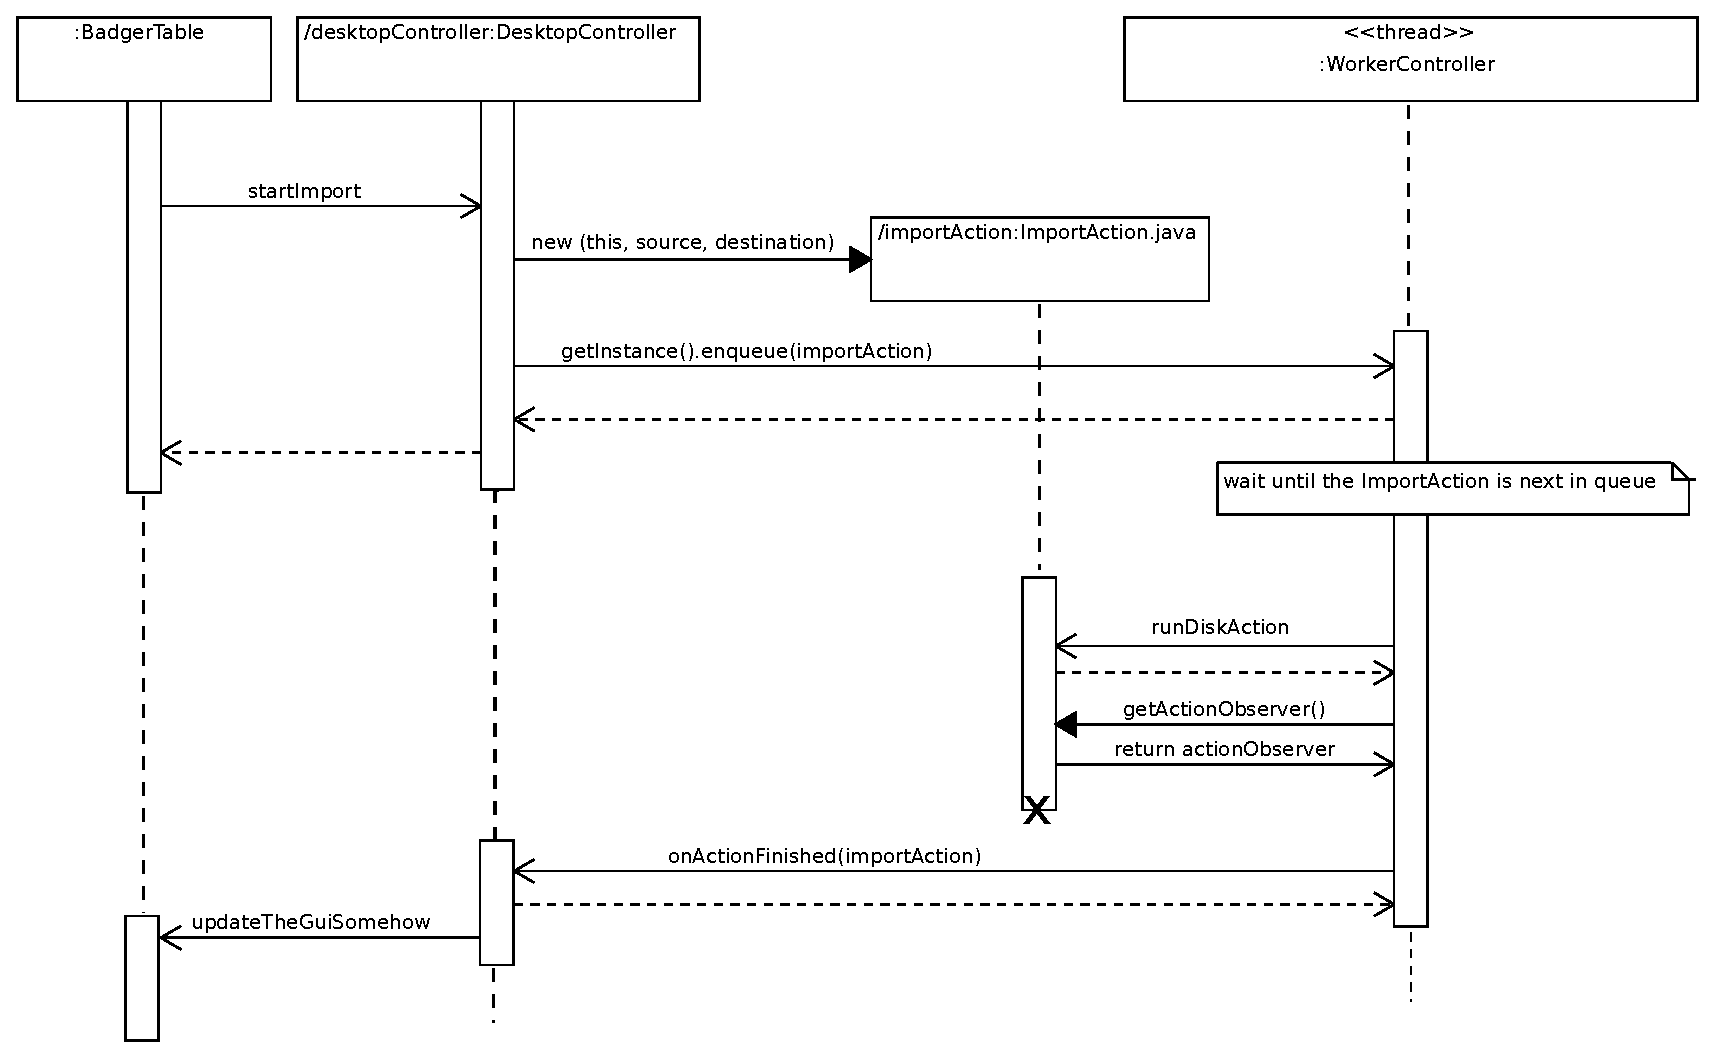
\includegraphics[width=1\textwidth]{figures/single_threaded_access.eps}
\caption{example of decoupling import from gui}
\label{fig:decouple_threads}
\end{figure}

Even when doing a seach the decoupling works pretty well: The
\textit{SearchAction} uses the VFS cores \textit{FindInFolderCallback} to update
the \textit{SearchController} which lives in the GUI thread every time finds an
entry.

\subsubsection{Search}
Searching files can be done in a separate Panel: After entering the search
string one is allowed to switch several flags like ``case sensitive'' or
``search subfolder'' and one can change the search folder.


\subsubsection{Keyboard and Mouse support}
One can navigate the list of entries by double clicking folders. The parent
folder can be accessed by double clicking ``..''. On right click on an entry the
user gets a menu depending on wheter she clicked on an file, folder or the empty
space. The right click in empty space reveals the same menu entries as the right
click on the parent folder. The only difference between file and folder menus
are the ``new folder'', ``paste'' and ``import'' actions, that are not allowed
on files.

The user is also allowed to select several files and folders from the list and
can then perform cut/copy or export on the selected items. 


\paragraph{Keyboard Shortcuts}
For keyboard wizards there are several keyboard shortcuts for doing the actions
on the selected entries.They keep to the general standards like F2 for renaming
or Ctrl+C for copy. The menus indicate the available shortcuts.
\paragraph{Drag \& Drop}
\subsection{Integration}

For the integration of the VFS core into the VFS Browser application almost
nothing had to be changed in the core. As the core is meant to be accessed by
only one thread at a time, the user interaction from the gui had to be bundled
into the \textit{WorkerController} and could be used from there without changes.
The only improvements on the core were done for the search, which allows some
wildcards that were not yet there in the first part of the project.



% PART III: Synchronization Server
% --------------------------------------

\section{Synchronization Server}

Synchronization Server is a command line server that allows synchronization of
virtual disks. It allows basic user management via VFS Browser, that includes
creating users and a login of created users. Logged in users can link local
disks to an account on the server via VFS Browser and then can connect to such
shared disks from an other client machine. Disks can also be created directly on
the server. When VFS Browser has a connection to the server, changes that occur
on the local disk will be propagated to the server which propagates these
changes to possibly other connected machines. If a user has
no connection to the Synchronization Server but operates on a disk that is
linked to a server instance the changes are recorded and are propagated as soon
as the connection is established next time. Thus synchronization server allows
seamless synchronization between several VFS Browser instances running on
different machines.



\subsection{Requirements}
Below one will find a list of the requirements implemented in this project.

\subsubsection {Requirements for the browser}
\begin{itemize}
  \item \emph{The browser should allow the user to create a new account or to log in to an existing account.}
  \item \emph{The browser should offer to switch to an online mode, and be able
  to operate without a connection to the server. }
  \item \emph{The browser should support binding an existing virtual disk to an active account.}
\end{itemize}  


\subsubsection {Requirements for the server}
\begin{itemize}
  \item \emph{The server should support registration of unique accounts. Each
  account includes name \& password.}
  \item \emph{The server should track changes to linked virtual disks of registered accounts and synchronize the
changes across the machines.}
\end{itemize}  


\subsubsection {Implemented Bonus Requirements}
\begin{itemize}
  \item \emph{Provide a set of mocked unit tests for your implementation.}

  \item \emph{Conflict Resolution: implement a conflict resolution scheme, so
  that concurrent changes to the same file are not lost (e.g. saving conflicting
  files as separate versions).}
  \item \emph{The browser is updating automatically when changes to the disk
  occur.}
  \item \emph{The server is able to synchronize changes, which are done
  simultaneously on the same account on different machines}
 
\end{itemize}

\subsubsection {Not Implemented Bonus Requirements}
\begin{itemize}
  \item \emph{File History: provide a history for files and an interface to
  restore a previous version}
 \item \emph{Incremental Changes: minimize the communication between the browser
 and the server by only transferring the parts of a file that changed.}
\end{itemize}

\subsection{Design}


\subsubsection{Scenarios}

Since milestone 3 VFS Browser can run in two different modes. Classic
mode\ref{fig:scenario_classic_mode} basically is the usage of virtual disks without any
server involved. Sync mode\ref{fig:22scenario_sync_mode} allows propagating
changes on a local disk (step 1) to a server (step 2). In
this mode changes are recorded in a journal, that gets sent over the wire when
the ``sync'' button is hit. To use a disk in sync mode one has to link a disk to
a server so that synchronization takes place between the local disk and the disk
on the server. The mechanism of journaling allows offline usage of a linked
disk, so that later on, when reconnecting to a server, local changes get
propagated to the disk on server side. Such changes on the
server side are sent to freshly attached clients that are working on the same
linked disk.

\begin{figure}[h!]
\centering
\includegraphics[width=1\textwidth]{figures/22scenario_classic_mode.eps}
\caption{scenario classic mode}
\label{fig:scenario_classic_mode}
\end{figure}

\begin{figure}[h!]
\centering
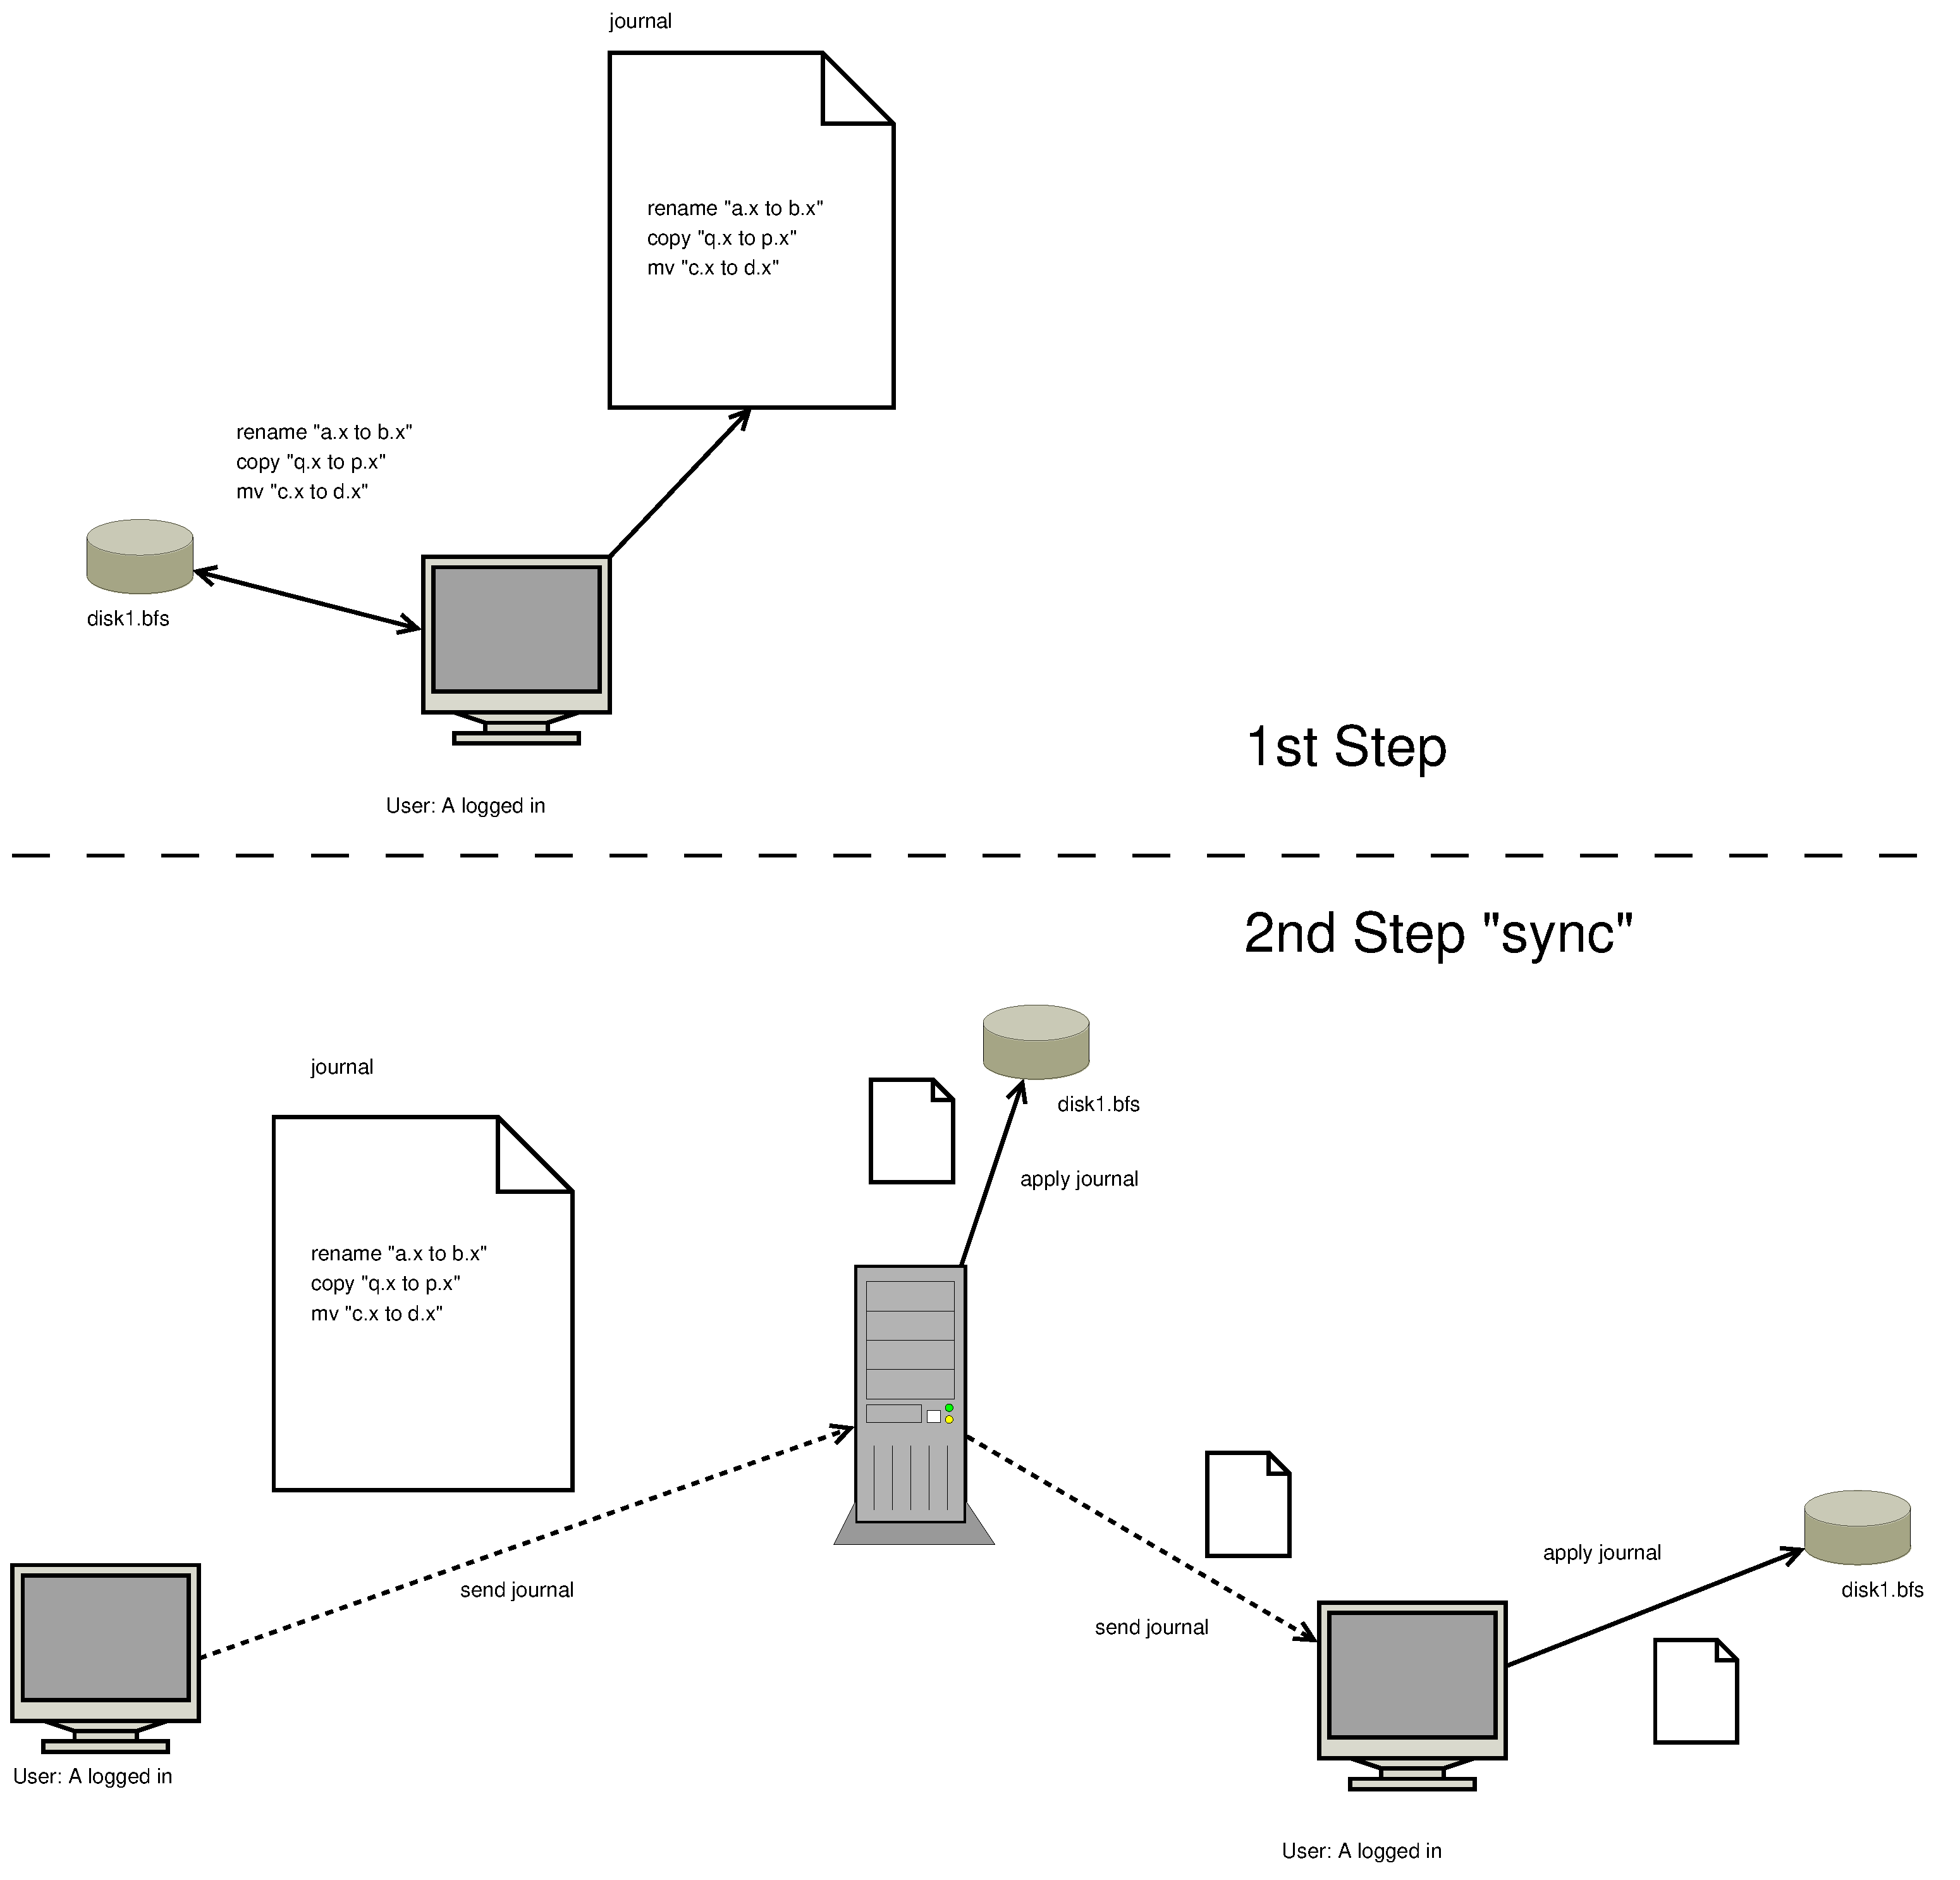
\includegraphics[width=1\textwidth]{figures/22scenario_sync_mode.eps}
\caption{scenario sync mode}
\label{fig:22scenario_sync_mode}
\end{figure}

\subsubsection{Technology}

\begin{figure}[h!]
\centering
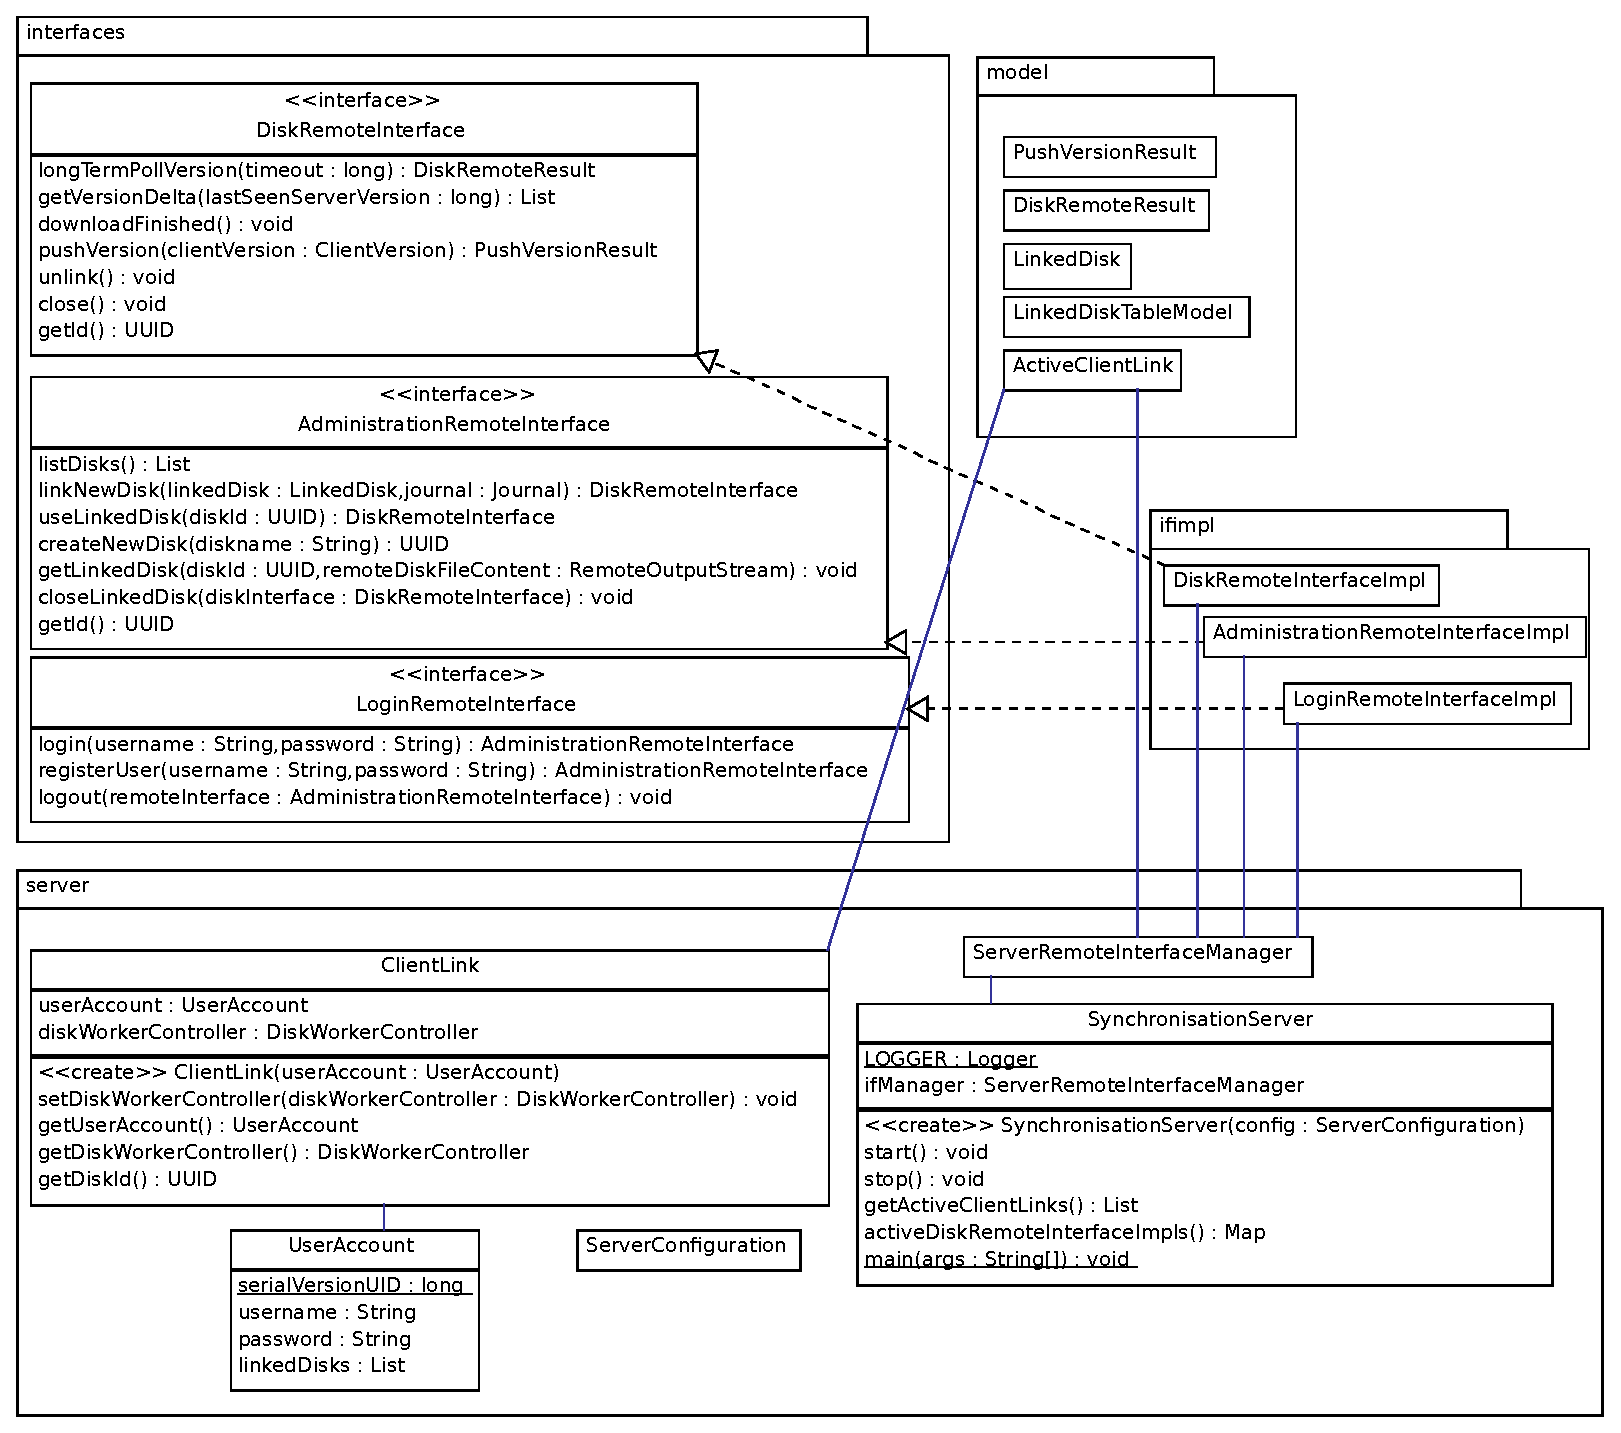
\includegraphics[width=1\textwidth]{figures/22Server.eps}
\caption{Server classes}
\label{fig:22server_classes}
\end{figure}

It was chosen to use JAVA RMI to establish client server
communication. Figure \ref{fig:22server_classes} shows the interfaces and
classes, that werde implemented to achieve communication. The three interfaces
\textit{LoginRemoteInterface, AdministrationRemoteInterface,
DiskRemoteInterface} hide the functionality to login/logout, create/link disks,
and push/pull journal updates for a disk. When a server starts up the
\textit{LoginRemoteInterfaceImpl} gets registered into the RMI registry and from
now on clients are allowed to connect through its interface. Every time a
client successfully logs in to the server a new
\textit{AdministrationRemoteInterfaceImpl} gets instantiated so that the client can link or open disks. Every time a disks
gets opened a new instance of \textit{DiskRemoteInterfaceImpl} gets
instantiated through which the client can synchronize local changes to the
corresponding server disk.


\subsubsection{User Management}
User management is kept very simple. Upon connecting to a server one can
create a new username/password or use a already existing one. Credentials are
being saved on server side together with its linked disks (see
\textit{UserAccount}).

\subsubsection{Synchronization}
Synchronization of disks is achieved by a simple journaling mechanism. Journals
get recorded when changes on a linked disk are made. These recorded journals get
sent to the server when ``sync'' button is hit. Changes that were done on a
remote client get synchronized to the local client upon login or periodically
with a long term polling mechanism. Figures \ref{fig:22uploadChanges} and
\ref{fig:22downloadChanges} show roughly, what happens when the ``sync'' button
is pressed: Through some indirection (\textit{DiskWorkerController and
RemoteWorkerController} that allow loose coupling of GUI, local disk and remote
communication threads) the client uploads/downloads \textit{Journal}s containing
\textit{JournalItem}s to/from the server which then get replayed on the other
side. Notice in particular the \textit{ModifyFileItem} that carries a special
variant of \textit{InputStream} to copy the binary data from a file to the other
side. A small drawback of this design is that while client is doing
synchronization no other actions can take place on its local disk. This includes
changing folder or simply all reading actions. Due to the lack of time it was
decided not to investigate further on that topic.

\begin{figure}[h!]
\centering
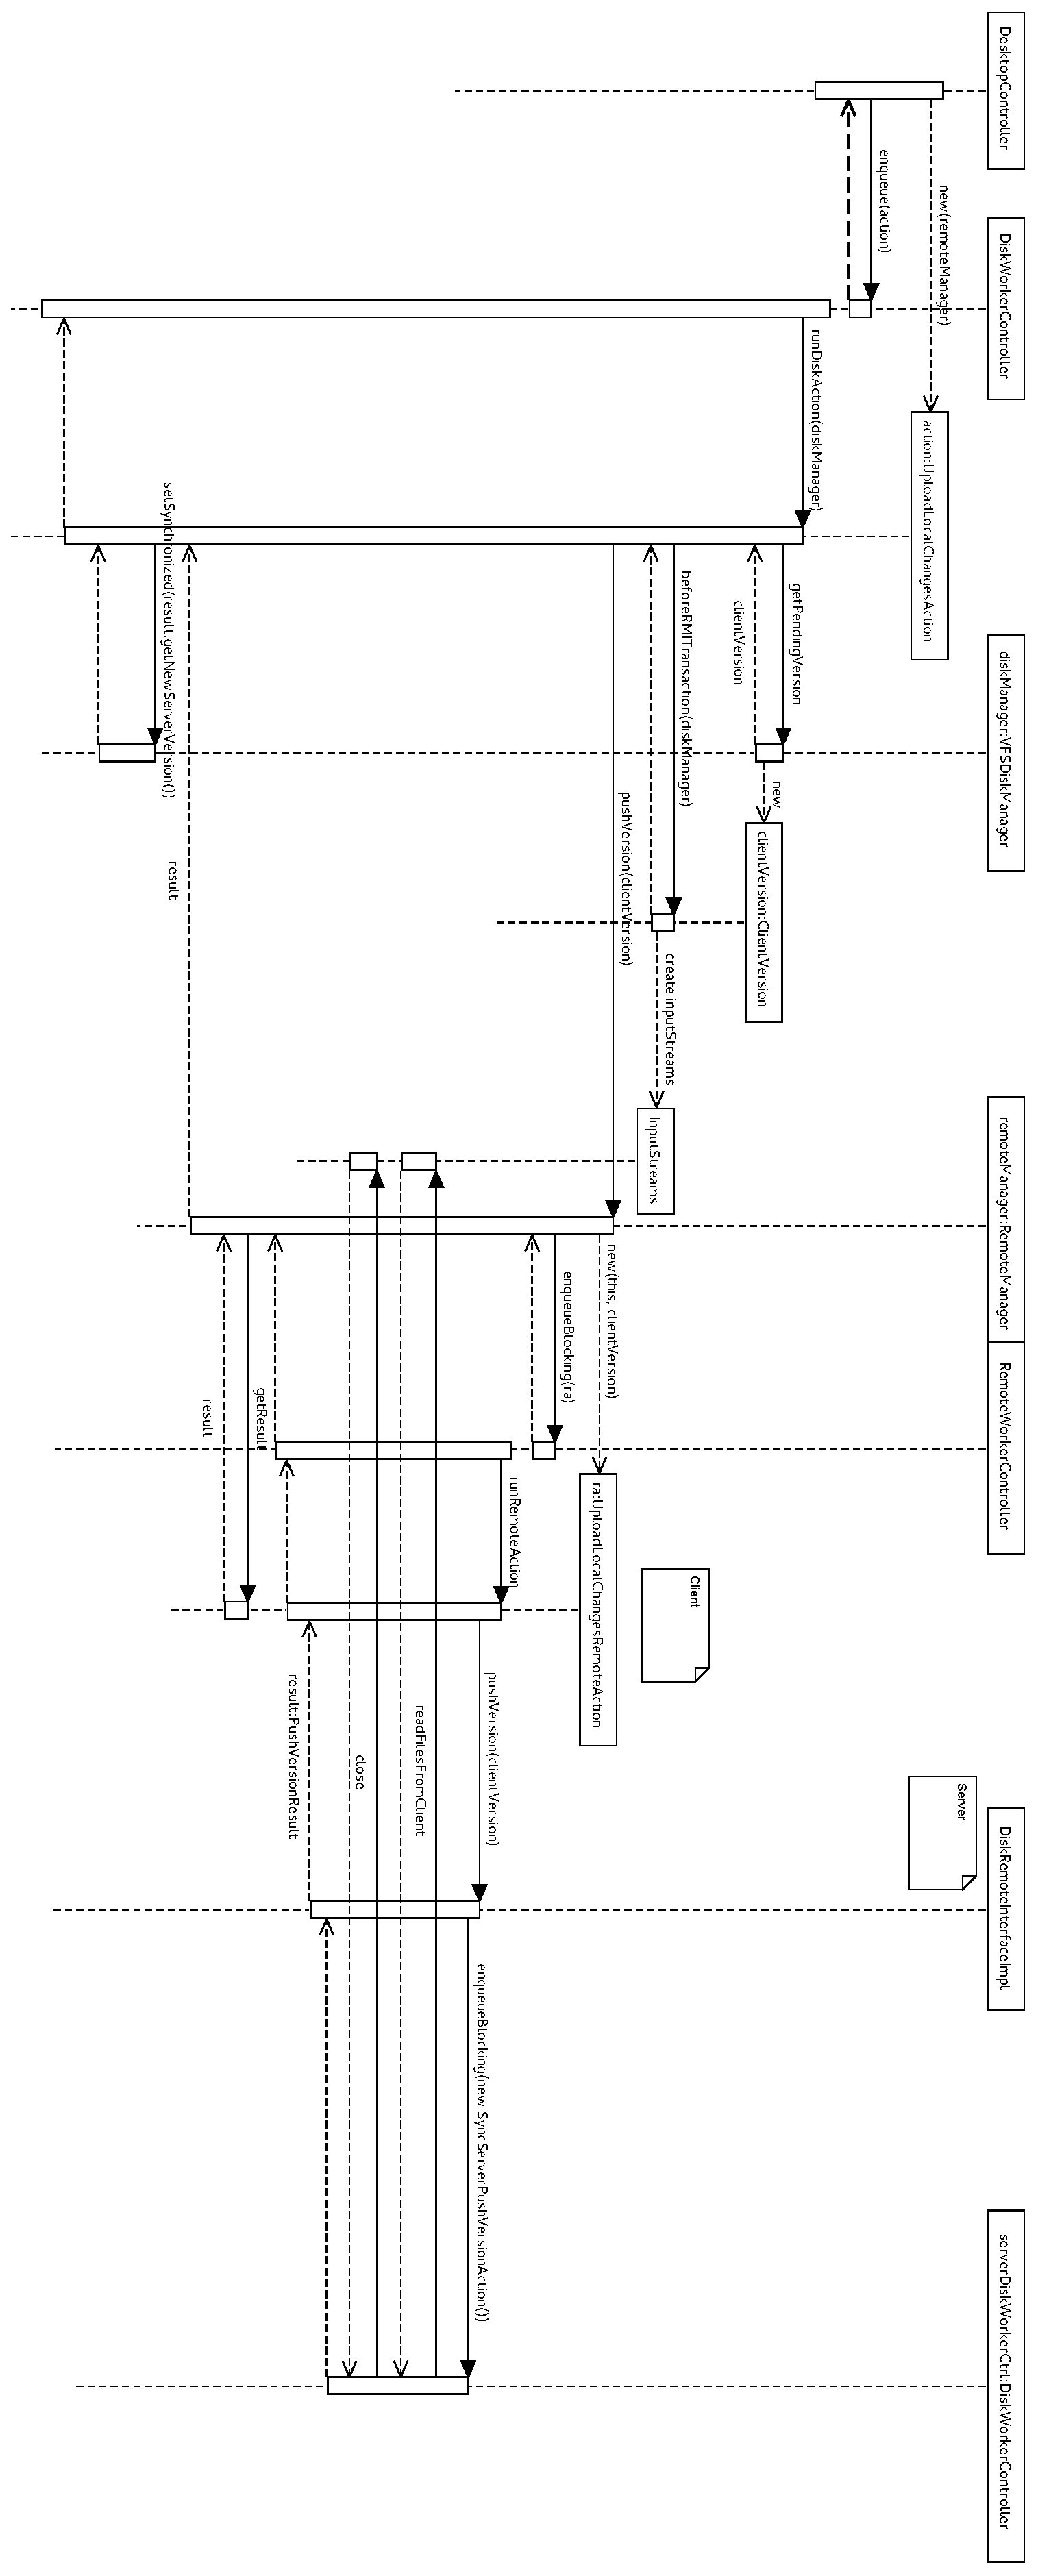
\includegraphics[height=\textheight,width=\textwidth,keepaspectratio]{figures/22uploadChanges.eps}
\caption{from click to upload changes to server}
\label{fig:22uploadChanges}
\end{figure}

\begin{figure}[h!]
\centering

\includegraphics[height=\textheight,width=\textwidth,keepaspectratio]{figures/22downloadChanges.eps}
\caption{from click to download changes from server}
\label{fig:22downloadChanges}
\end{figure}


\subsubsection{long term polling}
To make other clients aware that changes happened on their disk, a long term
polling mechanism was implemented. Clients start the
\textit{longTermPollVersion} method in the \textit{DiskRemoteInterface}. Upon
files get changed by a client the other clients that are currently connected to
the same disk get notified by returning the \textit{longTermPollVersion} method,
containing the actual server version, to which the clients now have to update.

\subsubsection{Journaling}
Figure \ref{fig:journaling_classes} gives an overview over the classes that
were implemented for journaling. The main thing to notice are the
\textit{JournalItem}s that carry out the operations they represent (e.g.
\textit{RenameEntryItem} renames a given entry to a new one.). For every disk a
logical version number is kept to make sure that no journals collide. Every time
a client synchronizes the last known server version number gets sent to the
server so that the server can decide which journals have to be propagated to the
client. Journals are kept inside the disk in a folder \verb|/.hidden/journals/|
and get deleted on the client side, as soon as the local changes are propagated
to the server. If file contents have to be transferred, they are copied and
saved under a uuid in a path that looks like \verb|/.hidden/journals/[journalnr]/file-[uuid]|.
Copying is done very quickly via a shallow copy mechanism, that had to be
implemented in VFS core. On the server side the disks mainly consist of the
whole journal from the beginning of time. With more time left for development
one could easily show a file history or even revert to any point in time.


\begin{figure}[h!]
\centering
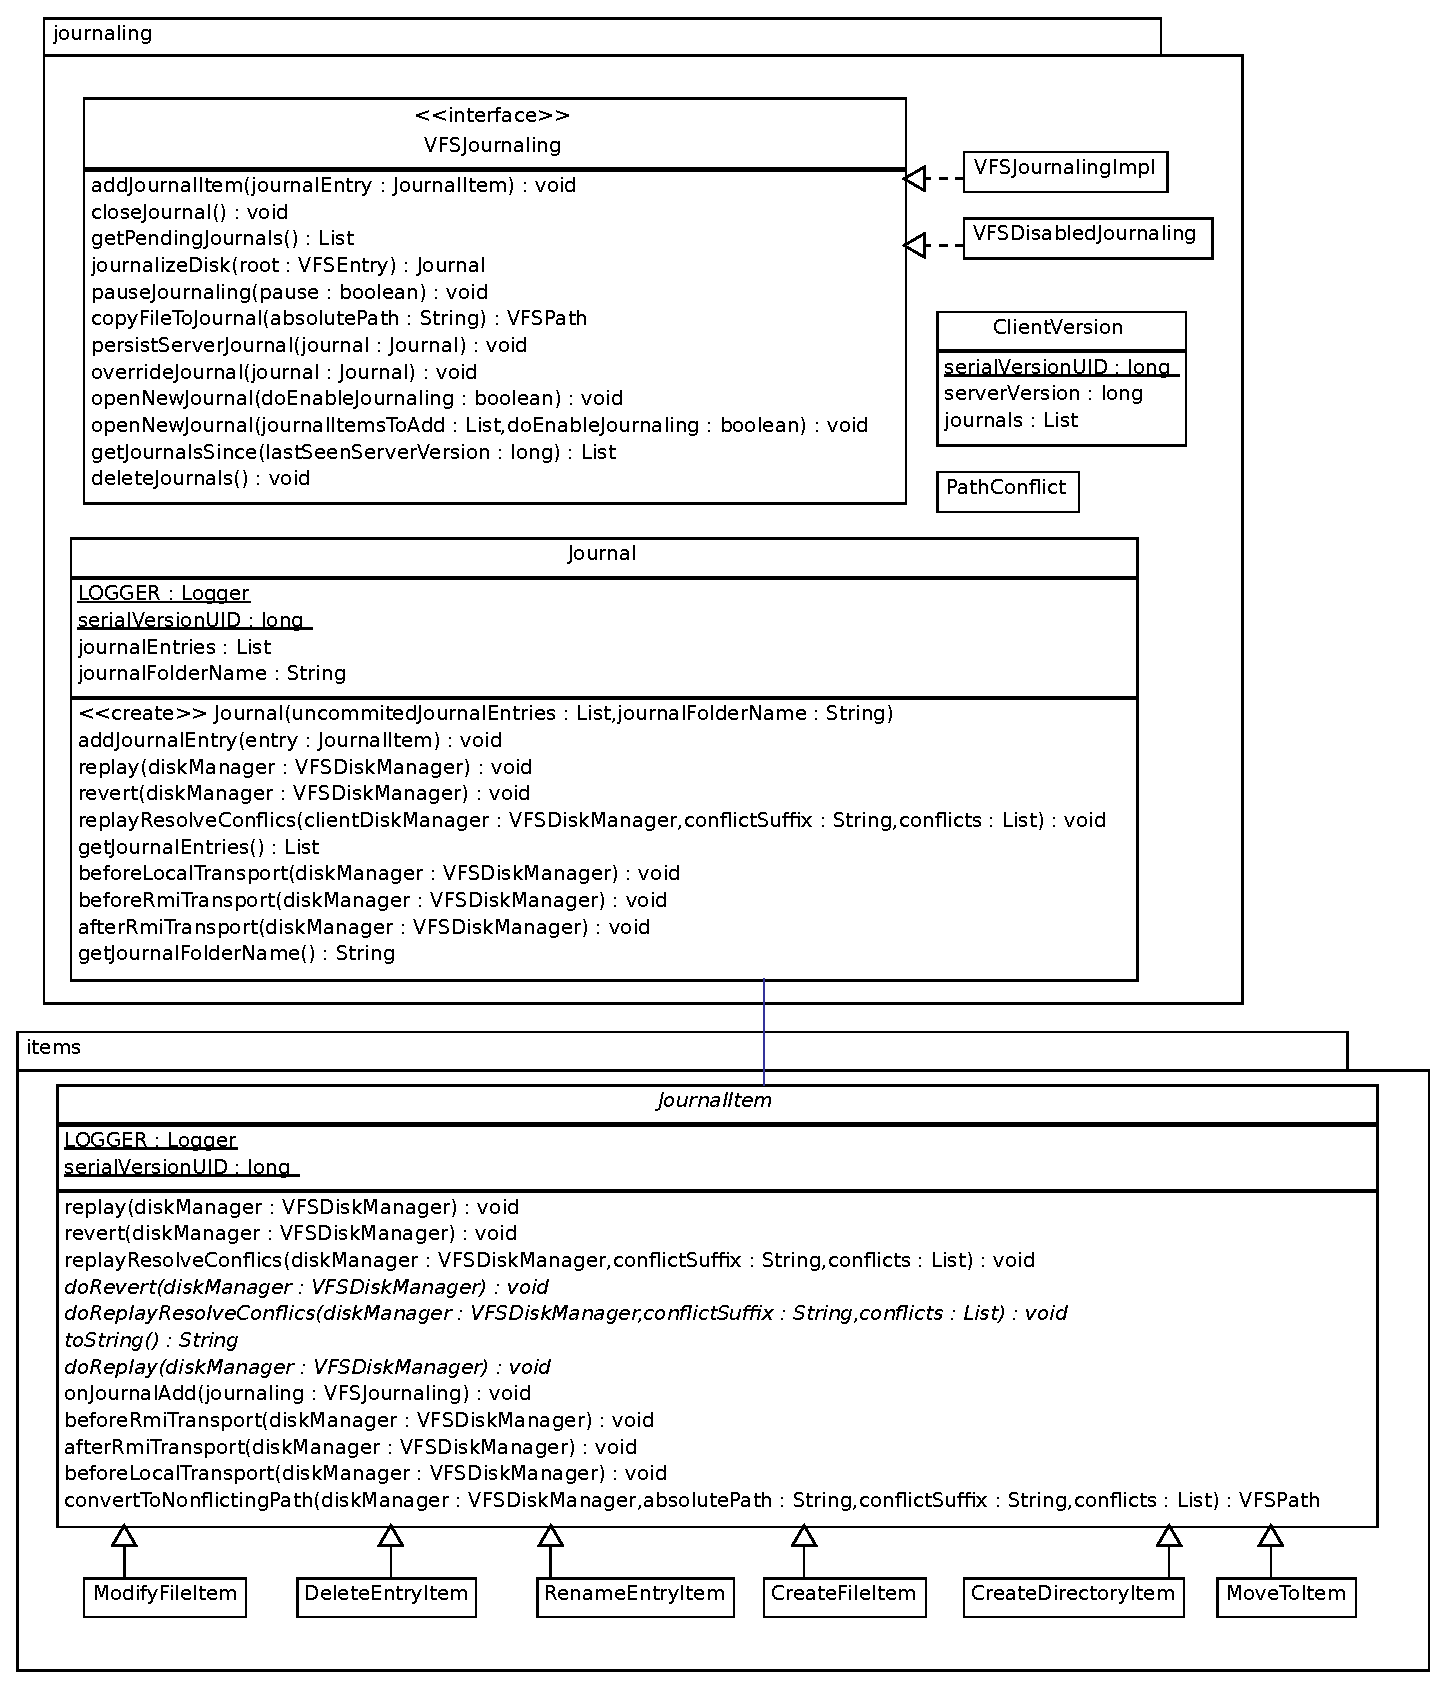
\includegraphics[width=1\textwidth]{figures/22Journaling.eps}
\caption{Journaling classes}
\label{fig:journaling_classes}
\end{figure}

\paragraph{Conflict resolution}
Based on the logical version numbers that are given to each journal the client
is able to do basic conflict resolution when it detects conflicting changes.
Files that got new content on the server while they were changed locally will be
renamed according to following scheme:

\begin{enumerate}
    \item revert local changes
  \item replay server journal (the client is in sync with server now)
  \item redo local changes
  \item push local changes to server
\end{enumerate}

\subsection{Integration}
To achieve goals like file synchronization, conflict management and history
browsing of a file, the interfaces developed in the second part of the project
were no longer good enough. Thus the journaling classes were integrated into the
core library. These classes help keeping track of the actions that take place on the
file system and are used to send changes on a local disk to the server. To have
journaling running as efficiently as possible the shallow copy mechanism was
developed. This mechanism does not copy the full file content but just has
reference counting on the datablock. The counters get increased/decreased
as copies are taken into the journal or deleted. This shallow-copy mechanism
only works, because files cannot be changed on the file system, they have to be renamed or deleted before
new content can be stored under the same name.




% PART IV: Quick Start Guide
% --------------------------------------

\section{Quick Start Guide}


\subsection{the eclipse project}
The project requires to be compiled with JAVA 7. It also depends on the maven
plugin which pulls in all the required libraries.

\subsection{Command line client}

The command line client allows the usage of the VFS core and is mainly intended
to test the basic functionalities. The console runs either in  management mode
or in file system mode. The management mode is entered automatically when
starting the command line client. It allows creating and opening virtual
disks. The file system mode is entered as soon as a virtual disk is opened.

%\textbf{TODO: DISCUSSION: sollen ganze ordner importiert und exportiert werden
%können? wird dies von der client-seite gehandelt?}

\subsubsection{startup}
The command line client can be started as follows:

\begin{verbatim}
java -jar VFSCore.jar ch.eth.jcd.badgers.vfs.ui.shell.VFSConsole
\end{verbatim}

or by starting \verb|ch.eth.jcd.badgers.vfs.ui.shell.VFSConsole| in eclipse.



This gives a console prompt where the following commands can be used in.

\subsubsection{commands}
Following commands can be used with the command line client in management mode:

\begin{itemize}
  \item{\textbf{create c:\textbackslash path\textbackslash to\textbackslash
  disk.bfs [size]}} creates virtual disk with a maximum quota of [size]
  megabytes on the host system. The file may grow up to [size] megabytes. There
  is currently no way to change encryption or compression by using the console
  application. By default no encryption and the LZ77 compression will be used.
  \item {\textbf{open c:\textbackslash path\textbackslash to\textbackslash
  disk.bfs}} opens filesystem mode for the given virtual disk
  \item {\textbf{exit}} exits the console program
\end{itemize}

following commands can be used in file system mode:

\begin{itemize}
  \item {\textbf{ls}} lists the contents of the current directory
  \item {\textbf{pwd}} shows the path to the current directory
  \item {\textbf{df}} shows the usage of the current virtual disk space
  \item {\textbf{cd dst}} changes current directory to \textit{dst} which must
  be either a child directory of the current path or ``..''
  \item {\textbf{find searchString}} lists absolute paths of all files
  containing \textit{searchString} in their file name
  \item {\textbf{mkdir dirName}} creates a new directory \textit{dirName} in the
  current path
  \item {\textbf{mkfile fileName}} creates a new empty file \textit{fileName} in
  the current path - this is rather not useful, as the ``import'' creates a
  file with content
  \item {\textbf{rm file}} deletes the entry denoted as \textit{file}, it must
  be a child of the current path
  \item {\textbf{cp src dst}} copies the \textit{src} file to \textit{dst} as a
  child of the current path
  \item {\textbf{mv src dst}} moves the \textit{src} file to \textit{dst}
  \item {\textbf{import ext\_src dst}} imports a \textit{ext\_src} from the
  host system to \textit{dst}
  \item {\textbf{export src ext\_src}} exports a \textit{src} file to the host
  system \textit{ext\_dst}
  \item {\textbf{find searchString}} lists all filesystem entries below the
  current entry containing \textit{searchString}
  \item {\textbf{dispose}} deletes the currently opened virtual disk
  \item {\textbf{close}} closes the file system mode, from now on management mode
  commands can be executed
\end{itemize}


\subsection{VFS Browser}
\subsubsection{startup}
The VFS Browser  can be started as follows:

\begin{verbatim}
java -jar VFSCore.jar ch.eth.jcd.badgers.vfs.ui.desktop.view.BadgerMainFrame
\end{verbatim}

or by starting \verb|ch.eth.jcd.badgers.vfs.ui.desktop.view.BadgerMainFrame| in eclipse.

Figures \ref{fig:01_quickstart}, \ref{fig:02_quickstart},
\ref{fig:03_quickstart}, \ref{fig:04_quickstart}, \ref{fig:05_quickstart} and
\ref{fig:06_quickstart} give a short overview of opening the browser and
importing the first folder. From there on the UI is pretty much self explanatory
of the features it exposes.

\begin{figure}[h!]
\centering
\includegraphics[width=1\textwidth]{figures/01_quickstart.png}
\caption{after startup, create a new disk}
\label{fig:01_quickstart}
\end{figure}

\begin{figure}[h!]
\centering
\includegraphics[width=1\textwidth]{figures/02_quickstart.png}
\caption{the disk creation wizard openes, one can choose the file, file size,
encryption and compression algorithms}
\label{fig:02_quickstart}
\end{figure}

\begin{figure}[h!]
\centering
\includegraphics[width=1\textwidth]{figures/03_quickstart.png}
\caption{the new disk gets created on the host filesystem and the user can
start importing files via Actions/Import\ldots}
\label{fig:03_quickstart}
\end{figure}

\begin{figure}[h!]
\centering
\includegraphics[width=1\textwidth]{figures/04_quickstart.png}
\caption{\ldots which triggers the import dialog, where the user can choose a
file or folder\ldots}
\label{fig:04_quickstart}
\end{figure}

\begin{figure}[h!]
\centering
\includegraphics[width=1\textwidth]{figures/05_quickstart.png}
\caption{after clicking ``OK'' the progress window appears\ldots}
\label{fig:05_quickstart}
\end{figure}

\begin{figure}[h!]
\centering
\includegraphics[width=1\textwidth]{figures/06_quickstart.png}
\caption{\ldots and finally the folder is imported after a couple of time.}
\label{fig:06_quickstart}
\end{figure}
\section{Glossary}

\paragraph{VFS core} The main Java library, that handles all the interaction
with virtual disks and importing/exporting/storing files. It is used by the
command line client and the GUI.

\paragraph{Virtual Disk} A virtual disk denotes a container file that is stored
on the host file system. A virtual disk can be opened with the software that is
developed during this project and stores the actual files. The file extension of
the virtual disk is ``*.bfs''.

\bibliographystyle{plain}
\bibliography{literature}
\end{document}
